\documentclass[13pt,a4paper]{article}
\usepackage[utf8]{vietnam}
\usepackage{amsmath}
\usepackage{amsfonts}
\usepackage{amssymb}
\usepackage[left=3.00cm, right=2.00cm, top=2.00cm, bottom=2.00cm]{geometry}
\usepackage{mathptmx}
\usepackage{graphicx}
\usepackage{float}
\usepackage{tikz}
\usepackage{hyperref}
\usetikzlibrary{calc}
\usepackage{indentfirst} %thu vien thut dau dong
\renewcommand{\baselinestretch}{1.2}% Gian dong 1.2
\setlength{\parskip}{6pt} %spacing after
\setlength{\parindent}{1cm} %thut dau dong moi doan
\usepackage{titlesec}
\titlespacing*{\section}{0pt}{0pt}{30pt} %Heading 1
\titleformat*{\section}{\fontsize{16pt}{0pt}\selectfont \bfseries \centering}

\titlespacing*{\subsection}{0pt}{10pt}{0pt} %Heading 2
\titleformat*{\subsection}{\fontsize{14pt}{0pt}\selectfont \bfseries}

\titlespacing*{\subsubsection}{0pt}{10pt}{0pt} %Heading 3
\titleformat*{\subsubsection}{\fontsize{13pt}{0pt}\selectfont \bfseries \itshape}

\titlespacing*{\paragraph}{0pt}{10pt}{0pt} %Heading 4
\titleformat*{\paragraph}{\fontsize{13pt}{0pt}\selectfont \itshape}

\renewcommand{\figurename}{\fontsize{12pt}{0pt}\selectfont \bfseries Hình}
\renewcommand{\thefigure}{\thesection.\arabic{figure}}
\usepackage{caption}
\captionsetup[figure]{labelsep=space}

\setcounter{secnumdepth}{4}
\setcounter{tocdepth}{4}

\begin{document}
\begin{titlepage}

\begin{center}
\vspace{-6pt} TRƯỜNG ĐẠI HỌC BÁCH KHOA THÀNH PHỐ HỒ CHÍ MINH\\
\textbf{\fontsize{16pt}{0pt}\selectfont BỘ MÔN VIỄN THÔNG}
\vspace{0.5cm}
\begin{figure}[H]
	\centering
	
\includegraphics[scale=.30]{image/bachkhoa.png}
\end{figure}
\vspace{0.5cm}
\fontsize{24pt}{0pt}\selectfont BÁO CÁO\\
\vspace{12pt}
\textbf{\fontsize{32pt}{0pt}\selectfont ĐỀ CƯƠNG LUẬN VĂN}
\vspace{1cm} 
\end{center}
\textbf{\fontsize{14pt}{0pt}\selectfont Đề tài:}
\begin{center}
	\textbf{\fontsize{20pt}{0pt}\selectfont ỨNG DỤNG CÔNG NGHỆ LORA VÀ MQTT VÀO NÔNG NGHIỆP THÔNG MINH}\\
\vspace{1.5cm}
\begin{table}[H]
	\centering
	\begin{tabular}{l l}
	\fontsize{14pt}{0pt}\selectfont Sinh viên thực hiện:  &\fontsize{14pt}{0pt}\selectfont LÊ ĐẠT - 1714121 \vspace{6pt}\\
	& Lớp DD17DV7 \vspace{6pt} \\
	\fontsize{14pt}{0pt}\selectfont Giảng viên hướng dẫn:  &\fontsize{14pt}{0pt}\selectfont TS. VÕ QUẾ SƠN\\
	\end{tabular}
\end{table}
\vspace{2cm}
\fontsize{14pt}{0pt}\selectfont TP Hồ Chí Minh, 4-2021
\end{center}
\end{titlepage}
\cleardoublepage
\addtocontents{toc}{\protect\thispagestyle{empty}}
\tableofcontents
\thispagestyle{empty}
\cleardoublepage

\pagenumbering{roman}
\section*{LỜI CẢM ƠN}
\addcontentsline{toc}{section}{\numberline {} LỜI CẢM ƠN}
\thispagestyle{empty}
Xin chân thành gửi lời cảm ơn tới TS. Võ Quế Sơn đã nhiệt tình giúp đỡ em trong suốt học kỳ đề cương vừa qua. Những lời nhận xét, góp ý, hướng dẫn của thầy đã giúp em có một hướng đi rõ ràng, cũng như hướng thực hiện đồ án này. Xin chân thành gửi lời cảm ơn tới toàn thể quý thầy cô trường Đại học Bách Khoa Thành phố Hồ Chí Minh đã giảng dạy, hướng dẫn và tạo mọi điều kiện, môi trường học tập tốt cho em trong những ngày tháng học tập tại trường. Đề tài thực tập được thực hiện bởi một thành viên, do thời gian có hạn, nên không thể tránh khỏi những thiếu sót. Rất mong nhận được sự góp ý của thầy để em học  hỏi thêm được nhiều kinh nghiệm và có thể thực hiện tốt hơn trong luận văn tốt nghiệp.

\vspace{6pt}
\hspace{7cm} TP. Hồ Chí Minh, ngày 20 tháng 04 năm 2021

\hspace{9cm}\textbf{Sinh viên thực hiện}

\vspace{2cm}
\hspace{9.85cm}\textbf{LÊ ĐẠT}
\cleardoublepage


\section*{DANH MỤC KÝ HIỆU VÀ CHỮ VIẾT TẮT}
\addcontentsline{toc}{section}{\numberline {} DANH MỤC KÝ HIỆU VÀ CHỮ VIẾT TẮT}
\cleardoublepage

\listoffigures
\addcontentsline{toc}{section}{\numberline {} DANH MỤC HÌNH VẼ}
\cleardoublepage

\listoftables
\addcontentsline{toc}{section}{\numberline {} DANH MỤC BẢNG BIỂU}
\cleardoublepage

\pagenumbering{arabic}

\section*{CHƯƠNG 1: GIỚI THIỆU}
\addcontentsline{toc}{section}{\numberline {} CHƯƠNG 1: GIỚI THIỆU}
\setcounter{section}{1}
\subsection{TỔNG QUAN}
\subsubsection{Đặt vấn đề}
IoT (Internet of things) được dịch sang tiếng Việt với nhiều tên gọi khác nhau như Internet Vạn Vật, Mạng lưới thiết bị kết nối Internet, Mạng lưới vạn vật kết nối Internet,… Trong đó, thuật ngữ được sử dụng phổ biến nhất là Internet Vạn Vật.\\
\indent IoT là một liên mạng với sự tham gia của nhiều thành phần. Trong đó, các thiết bị, phương tiện sẽ được bổ sung và tích hợp thêm các bộ phận điện tử, phần mềm cũng như các loại cảm biến giúp chúng vừa có thể thu thập dữ liệu, vừa có thể kết nối qua mạng máy tính để truyền và chia sẻ các dữ liệu đó. Hệ thống các thiết bị, phương tiện thông minh này sẽ tạo nên một cơ sở hạ tầng đáp ứng nhu cầu phát triển của xã hội thông tin.\\
\indent IoT là công nghệ đóng vai trò quan trọng và bắt đầu tác động đến nhiều lĩnh vực và ngành công nghiệp, từ sản xuất, y tế, truyền thông, năng lượng cho đến ngành nông nghiệp. IoT bao gồm cơ sở hạ tầng truyền thông cơ bản được sử dụng để kết nối các đối tượng thông minh từ cảm biến, phương tiện, thiết bị di động đến việc thu thập dữ liệu từ xa dựa trên phân tích thông minh, giao tiếp người dùng và cách mạng hóa ngành nông nghiệp.\\
\indent Bằng cách triển khai các công nghệ cảm biến và IoT trong thực tiễn nông nghiệp đã làm thay đổi mọi khía cạnh của phương pháp canh tác truyền thống. IoT giúp cải thiện các giải pháp về canh tác truyền thống như ứng phó với hạn hán, tối ưu hóa năng suất, tính phù hợp đất đai, tưới tiêu và kiểm soát dịch hại.\\
\indent MQTT (Đầy đủ là Message Queuing Telemetry Transport) là một giao thức gửi tín hiệu dạng publish/subscribe. Chúng được sử dụng cho các thiết bị Internet of Things – IoT. Tín hiệu truyền đi với băng thông thấp, có độ tin cậy cao và khả năng sử dụng được trong mạng lưới thiếu ổn định. Bởi vì giao thức MQTT này sử dụng băng thông khá thấp trong môi trường có độ trễ cao nên nó là một giao thức lý tưởng cho các ứng dụng M2M (Machine to Machine).\\
\indent Công nghệ LoRa , được phát triển bởi Semtech , là một giao thức không dây mới được thiết kế để truyền thông tầm xa, năng lượng thấp. Giao thức cung cấp loại khả năng liên lạc mà các thiết bị thông minh cần có, và Liên minh LoRa đang hoạt động để đảm bảo khả năng tương tác giữa nhiều mạng trên toàn quốc.\\
\indent Một phần của phổ LoRa sử dụng thể hiện ít nhiễu điện từ, do đó tín hiệu có thể kéo dài một khoảng cách xa, thậm chí đi qua các tòa nhà, với rất ít năng lượng. Điều này phù hợp với các thiết bị IoT với dung lượng pin hạn chế. Điều đó cũng có nghĩa là các tinh thể chi phí thấp hơn có thể được sử dụng, do đó, việc xây dựng LoRa thành các thiết bị rẻ hơn.\\
\indent Mỗi gateway LoRa có thể xử lý hàng triệu node. Điều đó, cộng với thực tế là các tín hiệu có thể kéo dài khoảng cách đáng kể, có nghĩa là cần ít cơ sở hạ tầng mạng hơn, do đó làm cho việc xây dựng mạng LoRa rẻ hơn. Các mạng LoRa có thể được đặt cùng với các thiết bị liên lạc khác, như các tháp điện thoại di động, làm giảm đáng kể các hạn chế xây dựng.\\
\indent Các tính năng khác của LoRa cũng khiến nó trở nên lý tưởng cho IoT. LoRa sử dụng thuật toán tốc độ dữ liệu thích ứng để giúp tối đa hóa tuổi thọ pin và dung lượng mạng của thiết bị. Các giao thức của nó bao gồm nhiều lớp mã hóa, ở cấp độ mạng, ứng dụng và thiết bị, cho phép liên lạc an toàn. Tính hai chiều của giao thức hỗ trợ các thông điệp quảng bá, cho phép chức năng cập nhật phần mềm.\\
\indent Sự phát triển của Internet of Things bị giới hạn bởi dung lượng của mạng, bởi khả năng hoạt động của thiết bị mà không cần thay pin và bởi khả năng mã hóa truyền dẫn bí mật. Các tính năng được tích hợp trong LoRa cung cấp tất cả các khả năng này và sẽ cho phép sự phát triển rộng rãi của IoT.\\
\indent Với công nghệ Lora , chúng ta có thể truyền dữ liệu với khoảng cách lên hàng km mà không cần các mạch khuếch đại công suất; từ đó giúp tiết kiệm năng lượng tiêu thụ khi truyền/nhận dữ liệu. Do đó, LoRa có thể được áp dụng rộng rãi trong các ứng dụng thu thập dữ liệu như sensor network trong đó các sensor node có thể gửi giá trị đo đạc về trung tâm cách xa hàng km và có thể hoạt động với battery trong thời gian dài trước khi cần thay pin.\\
\\

\indent Nhận thấy những ưu điểm của Lora, giao thức MQTT và những ứng dụng vô cùng thực tế của IoT trong nông nghiệp. Chính vì vậy mục tiêu của đề tài tạo ra mạng kết nối với các thiết bị dùng để điều khiển, các cảm biến thu thập dữ liệu, vẽ đồ thị trạng thái dựa trên dữ liệu thu thập được từ cảm biến thông qua mạng LoRa và giao thức MQTT.
\subsubsection{Tình hình nghiên cứu trong nước}
Qua tìm hiểu về tình hình nghiên cứu, trong nước rất ít dự án ứng dụng công nghệ LoRa đưa vào thực tế. Tuy nhiên cũng có rất nhiều dự án, công trình đã và đang được nghiên cứu:
\begin{itemize}
	\item Lê Đình Vương, MSSV 41204661, đề tài luận văn "Thu thập và quản lí dữ liệu thông qua mạng LoRa", Đại học Bách Khoa TP.HCM, tháng 6 năm 2017.
	\item Nguyễn Quốc Anh, MSSV 21300108, đề tài luận văn "Thiết kế hệ thống đo lường chất lượng hồ nuôi tôm sử dụng công nghệ LoRa", Đại học Bách Khoa TP.HCM, tháng 5 năm 2018.
\end{itemize}
\subsubsection{Tình hình nghiên cứu ngoài nước}
Hiện nay có nhiều cá nhân, công ty nghiên cứu phát hành sản phẩm LoRa mộthay nhiều kênh truyền dựa trên chipset của Semtech. Các công trình nghiên cứu:
\begin{itemize}
	\item Đề tài “A DIY low-cost LoRa gateway” của Giáo sư Phạm Công Đức, trường đại học Paul, Pháp sử dụng chip SX1276 của Semtech với Gateway một kênh truyền.
	\item Module LoRaWan IXM-LPWA-800-16-K9 của Cisco cho các ứng dụng cần công suất thấp, diện tích phủ rộng lớn như tracking vật thể, đo nước hay khí.
\end{itemize}
\subsection{NHIỆM VỤ}
\subsubsection{Mục tiêu đề tài}
Thực hiện truyền dữ liệu nhiệt độ, độ ẩm từ End-node thông qua LoRa về Gateway, Gateway chuyển tiếp dữ liệu thông qua giao thức MQTT về App điện thoại thông minh.\\
\indent Truyền lệnh điều khiển bật/tắt đèn từ App điện thoại thông minh về Gateway thông qua giao thức MQTT, Gateway chuyển tiếp đến End-node thực hiện lệnh thông qua LoRa
\subsubsection{Yêu cầu đề tài}
\begin{itemize}
	\item \textbf{Nội dung 1:} Tìm hiểu module RF UART Lora E32-TTL-100 SX1278 SEMTECH
	\item \textbf{Nội dung 2:} Tìm hiểu MQTT và LoRa
	\item \textbf{Nội dung 3:} Xây dựng App Android
\end{itemize}
\subsubsection{Kế hoạch thực hiện}
\begin{figure}[H]
	\centering
	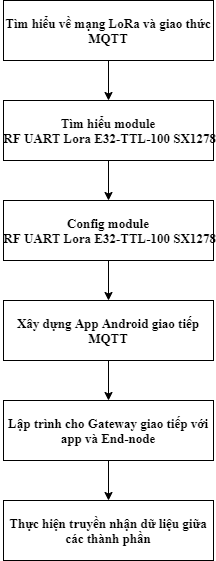
\includegraphics[scale=.5]{Chapter 1/image chapter 1/kehoachthuchien.png}
	\caption[Kế hoạch thực hiện]{Kế hoạch thực hiện}
	\label{hinh11}
\end{figure}


\section*{CHƯƠNG 2: LÝ THUYẾT}
\addcontentsline{toc}{section}{\numberline {} CHƯƠNG 2: LÝ THUYẾT}
\setcounter{section}{2}
\setcounter{figure}{0}
\setcounter{subsection}{0}
\subsection{CÔNG NGHỆ LORA}
\subsubsection{Khái niệm}
LoRa là viết tắt của Long Range Radio được nghiên cứu và phát triển bởi Cycleo và sau này được mua lại bởi công ty Semtech năm 2012. Với công nghệ này, chúng ta có thể truyền dữ liệu với khoảng cách lên hàng km mà không cần các mạch khuếch đại công suất; từ đó giúp tiết kiệm năng lượng tiêu thụ khi truyền/nhận dữ liệu. Do đó, LoRa có thể được áp dụng rộng rãi trong các ứng dụng thu thập dữ liệu như sensor network trong đó các sensor node có thể gửi giá trị đo đạc về trung tâm cách xa hàng km và có thể hoạt động với battery trong thời gian dài trước khi cần thay pin.\\
\indent Với tầm xa ,nền tảng không dây công suất thấp là sự lựa chọn công nghệ phổ biến hiện hành để xây dựng mạng iot trên thế giới ứng dụng iot thông minh đã cải thiện theo cách tương tác và giải quết giải quyết một số thách thức lớn nhất mà các thành phố và cộng đồng đang phải đối mặt :biến đổi khí hậu ,kiểm soát ô nhiễm cảnh báo thiên tai và cứu mạng .Kinh doanh cũng được hưởng lợi thông qua cũng như giảm được chi phí. Đây là RF công nghệ không dây được tích hợp vào xe ô tô, đèn đường , sản xuất thiết bị , đồ gia dụng thiết bị đeo được bất cứ điều gì , thực sự . Công nghệ Lora đang làm thế giới ta một hành tinh thông minh\\
\indent Dưới đây là hình ảnh để bạn hiểu rõ nét về tầm xa của Lora:
\begin{figure}[H]
	\centering
	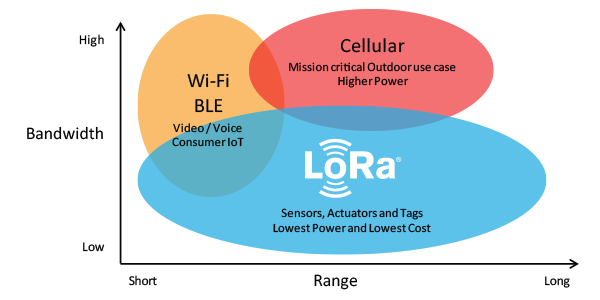
\includegraphics[scale=.5]{Chapter 2/image chapter 2/tamxaLoRa.png}
	\caption[Ảnh minh hoạ tầm xa LoRa]{Ảnh minh hoạ tầm xa LoRa}
	\label{hinh21}
\end{figure}
\subsubsection{Nguyên lý hoạt động}
LoRa sử dụng kỹ thuật điều chế gọi là Chirp Spread Spectrum. Có thể hiểu nôm na nguyên lý này là dữ liệu sẽ được băm bằng các xung cao tần để tạo ra tín hiệu có dãy tần số cao hơn tần số của dữ liệu gốc (cái này gọi là chipped); sau đó tín hiệu cao tần này tiếp tục được mã hoá theo các chuỗi chirp signal (là các tín hiệu hình sin có tần số thay đổi theo thời gian; có 2 loại chirp signal là up-chirp có tần số tăng theo thời gian và down-chirp có tần số giảm theo thời gian; và việc mã hoá theo nguyên tắc bit 1 sẽ sử dụng up-chirp, và bit 0 sẽ sử dụng down-chirp) trước khi truyền ra anten để gửi đi.\\
\indent Theo Semtech công bố thì nguyên lý này giúp giảm độ phức tạp và độ chính xác cần thiết của mạch nhận để có thể giải mã và điều chế lại dữ liệu; hơn nữa LoRa không cần công suất phát lớn mà vẫn có thể truyền xa vì tín hiệu Lora có thể được nhận ở khoảng cách xa ngay cả độ mạnh tín hiệu thấp hơn cả nhiễu môi trường xung quanh.\\
\indent Băng tần làm việc của LoRa từ 430MHz đến 915MHz cho từng khu vực khác nhau trên thế giới:
\begin{itemize}
	\item 430MHz cho châu Á
	\item 780MHz cho Trung Quốc
	\item 433MHz hoặc 866MHz cho châu Âu
	\item 915MHz cho USA
\end{itemize}

\indent Nhờ sử dụng chirp signal mà các tín hiệu LoRa với các chirp rate khác nhau có thể hoạt động trong cùng 1 khu vực mà không gây nhiễu cho nhau. Điều này cho phép nhiều thiết bị LoRa có thể trao đổi dữ liệu trên nhiều kênh đồng thời (mỗi kênh cho 1 chirprate). Công nghệ điều chế trải phổ trải phổ Chirp (Chirp Spread Spectrum) với sự biến đổi tuyến tính của tần số theo thời gian để mã hóa thông tin. Bởi vì sự tuyến tính của xung trải phổ, độ lêch tần số giữa cácthiết bị thu và phát tương ứng với độ lệch thời gian, dễ dàng bị loại bỏ trong giảimã. Điều này giúp cho giảm ảnh hưởng của hiệu ứng Doppler. Độ lệch tần số giữathu và phát có thể đạt đến 20\% băng thông mà không ảnh hưởng hiệu suất mã hóa.Máy thu LoRa có thể cung cấp độ nhạy lên tới -148dBm. Một số tính năng chính:
\begin{itemize}
	\item Khả năng chống lại nhiễu cố ý và không cố ý - đặc điểm quan trọng đối với thông tin trong các vùng đông đúc như thành phố.
	\item Có khả năng loại bỏ hoặc giảm nhẹ ảnh hưởng của truyền lan đa đường (multi path fading).
	\item Có khả năng chống lại hiệu ứng Doppler (độ lệch tần số giữa thu và phát có thể đạt tới 20\% băng thông).
	\item Có thể chia sẻ cùng băng tần với các người dùng khác, nhờ tính chất tín hiệu giống như tạp âm của nó.
	\item Cho mức độ riêng tư nhất định nhờ tính chất của điều chế trải phổ, người ngoài khó có thể đánh cắp được dữ liệu vì không nắm được sự thay đổi về tần số của tín hiệu.
\end{itemize}

\indent Một vài thông số cho việc tùy biến trong điều chế LoRa:
\begin{itemize}
	\item \textbf{Hệ số trải phổ (SF):} SF có giá trị trong khoảng từ 6 đến 12. SF = 6 là mode cho tốc độ truyền bit cao nhất. Trong khi đó hệ số trải phổ càng tăng dẫn đến độ nhạy máy thu càng tăng.
	\item \textbf{Tỉ lệ mã hóa (CR):} Modem LoRa sử dụng Cyclic Error Coding để phát hiện và sửa lỗi. Error Coding thực hiện khi truyền tải trong không khí.
	\item \textbf{Băng thông (BW):} Tăng băng thông dẫn tới tăng tốc độ dữ liệu, dẫn tới giảm thời gian truyền dẫn, giảm độ nhạy.
\end{itemize}
\subsubsection{Module thu phát RF UART E32-TTL-100}
\begin{figure}[H]
	\centering
	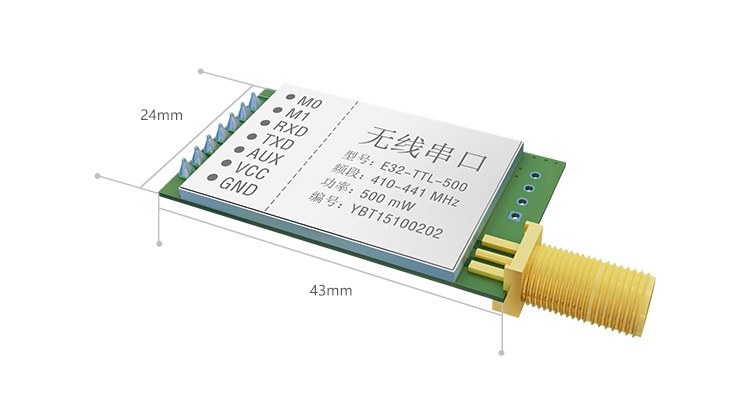
\includegraphics[scale=.4]{Chapter 2/image chapter 2/E32.jpg}
	\caption[Module RF UART E32-TTL-100]{Module RF UART E32-TTL-100}
	\label{hinh22}
\end{figure}
Mạch thu phát RF UART Lora SX1278 433Mhz 3000m sử dụng chip SX1278 của nhà sản xuất SEMTECH chuẩn giao tiếp LORA (Long Range), chuẩn LORA mang đến hai yếu tố quan trọng là tiết kiệm năng lượng và khoảng cách phát siêu xa ( Ultimate long range wireless solution), ngoài ra nó còn có khả năng cấu hình để tạo thành mạng nên hiện tại được phát triển và sử dụng rất nhiều trong các nghiên cứu về IoT.\\
\indent Mạch thu phát RF UART Lora SX1278 433Mhz 3000m được tích hợp phần chuyển đổi giao tiếp SPI của SX1278 sang UART giúp việc giao tiếp và sử dụng rất dễ dàng, chỉ cần kết nối với Software của hãng để cấu hình địa chỉ , tốc độ và công suất truyền là có thể sử dụng.\\
\subsection{GIAO THỨC MQTT}
\subsubsection{Khái niệm}
MQTT (\textbf{Message Queuing Telemetry Transport}) là giao thức truyền thông điệp (message) theo mô hình publish/subscribe (cung cấp /thuê bao), được sử dụng cho các thiết bị IoT với băng thông thấp, độ tin cậy cao và khả năng được sử dụng trong mạng lưới không ổn định. Nó dựa trên một Broker (tạm dịch là “Máy chủ môi giới”) “nhẹ” (khá ít xử lý) và được thiết kế có tính mở (tức là không đặc trưng cho ứng dụng cụ thể nào), đơn giản và dễ cài đặt.\\
\indent MQTT là lựa chọn lý tưởng trong các môi trường như:
\begin{itemize}
	\item Những nơi mà giá mạng viễn thông đắt đỏ hoặc băng thông thấp hay thiếu tin cậy.
	\item Khi chạy trên thiết bị nhúng bị giới hạn về tài nguyên tốc độ và bộ nhớ.
	\item Bởi vì giao thức này sử dụng băng thông thấp trong môi trường có độ trễ cao nên nó là một giao thức lý tưởng cho các ứng dụng M2M (Machine to Machine).
\end{itemize}

\indent MQTT cũng là giao thức được sử dụng trong Facebook Messenger\\
\indent \textbf{Lịch sử hình thành}
\begin{itemize}
	\item MQTT được phát minh bởi Andy Stanford - Clark (IBM) và Arlen Nipper (EUROTECH) cuối năm 1999 khi mà nhiệm vụ của họ là tạo ra một giao thức sao cho sự hao phí năng lượng và băng thông là thấp nhất để kết nối đến đường ống dẫn dầu thông qua sự kết nối của vệ tinh.
	\item Năm 2011, IBM và Eurotech đã trao lại MQTT cho một dự án của Eclipse có tên là Paho.
	\item Năm 2013 MQTT đã được đệ trình lên OASIS (Organization for the Advancement of Structured Information Standards) để chuẩn hóa.
\end{itemize}
\begin{figure}[H]
	\centering
	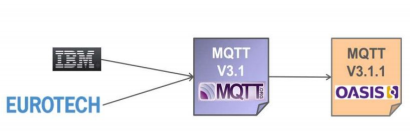
\includegraphics[scale=.7]{Chapter 2/image chapter 2/lichsuMQTT.png}
	\caption[Lịch sử hình thành MQTT]{Lịch sử hình thành MQTT}
	\label{hinh25}
\end{figure}
\subsubsection{Cơ chế hoạt động của MQTT theo mô hình Pub/Sub}
\textbf{Tính chất:}
\begin{itemize}
	\item Space decoupling (Không gian tách biệt).
	\item Time decoupling (Thời gian tách biệt).
	\item Synchronization decoupling (Sự đồng bộ riêng rẽ).
\end{itemize}

\indent \textbf{Đặc điểm riêng:}
\begin{itemize}
	\item MQTT sử dụng cơ chế lọc thông điệp dựa vào tiêu đề (subject-based).
	\item MQTT có một tầng gọi là chất lượng dịch vụ (Quality of Services – QoS). Nó giúp cho dễ dàng nhận biết được là message có được truyền thành công hay không.
\end{itemize}

\indent \textbf{Cơ chế tổng quan}
\begin{figure}[H]
	\centering
	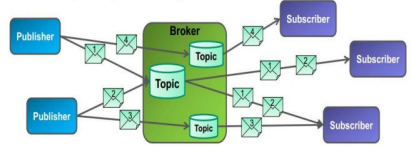
\includegraphics[scale=.7]{Chapter 2/image chapter 2/cochetongquanMQTT.png}
	\caption[Cơ chế tổng quan MQTT]{Cơ chế tổng quan MQTT}
	\label{hinh27}
\end{figure}
MQTT hoạt động theo cơ chế client/server, nơi mà mỗi cảm biến là một khách hàng (client) và kết nối đến một máy chủ, có thể hiểu như một Máy chủ môi giới (broker), thông qua giao thức TCP (Transmission Control Protocol). Broker chịu trách nhiệm điều phối tất cả các thông điệp giữa phía gửi đến đúng phía nhận.\\
\indent MQTT là giao thức định hướng bản tin. Mỗi bản tin là một đoạn rời rạc của tín hiệu và broker không thể nhìn thấy. Mỗi bản tin được publish một địa chỉ, có thể hiểu như một kênh (Topic). Client đăng kí vào một vài kênh để nhận/gửi dữ liệu, gọi là subscribe. Client có thể subscribe vào nhiều kênh. Mỗi client sẽ nhận được dữ liệu khi bất kỳ trạm nào khác gửi dữ liệu vào kênh đã đăng ký. Khi một client gửi một bản tin đến một kênh nào đó gọi là publish.\\
\indent \textbf{Kiến trúc thành phần}
\begin{figure}[H]
	\centering
	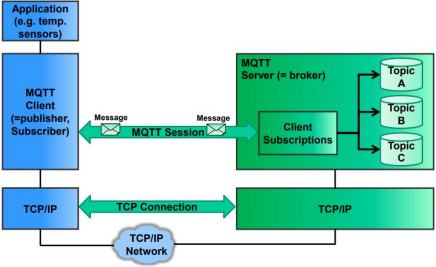
\includegraphics[scale=.7]{Chapter 2/image chapter 2/kientrucMQTT.png}
	\caption[Kiến trúc thành phần MQTT]{Kiến trúc thành phần MQTT}
	\label{hinh28}
\end{figure}
Thành phần chính của MQTT là Client (Publisher/Subscriber), Server (Broker), Sessions (tạm dịch là Phiên làm việc), Subscriptions và Topics.\\
\indent \textit{MQTT Client (Publisher/Subscriber):} Clients sẽ subscribe một hoặc nhiều topics để gửi và nhận thông điệp từ những topic tương ứng.\\
\indent \textit{MQTT Server (Broker):} Broker nhận những thông tin subscribe (Subscriptions) từ client, nhận thông điệp, chuyển những thông điệp đến các Subscriber tương ứng dựa trên Subscriptions từ client.\\
\indent \textit{Topic:} Có thể coi Topic là một hàng đợi các thông điệp, và có sẵn khuôn mẫu dành cho Subscriber hoặc Publisher. Một cách logic thì các topic cho phép Client trao đổi thông tin với những ngữ nghĩa đã được định nghĩa sẵn. Ví dụ: Dữ liệu cảm biến nhiệt độ của một tòa nhà.\\
\indent \textit{Session:} Một session được định nghĩa là kết nối từ client đến server. Tất cả các giao tiếp giữa client và server đều là 1 phần của session.\\
\indent \textit{Subscription:} Không giống như session, subscription về mặt logic là kết nối từ client đến topic. Khi đã subscribe một topic, Client có thể nhận/gửi thông điệp (message) với topic đó.



\section*{CHƯƠNG 3: MCU VÀ PHẦN CỨNG ĐƯỢC SỬ DỤNG TRONG THỰC TẬP}
\addcontentsline{toc}{section}{\numberline {} CHƯƠNG 3: MCU VÀ PHẦN CỨNG ĐƯỢC SỬ DỤNG TRONG THỰC TẬP}
\setcounter{section}{3}
\setcounter{figure}{0}
\setcounter{subsection}{0}
\subsection{ARDUINO NANO CH340}
\begin{figure}[H]
	\centering
	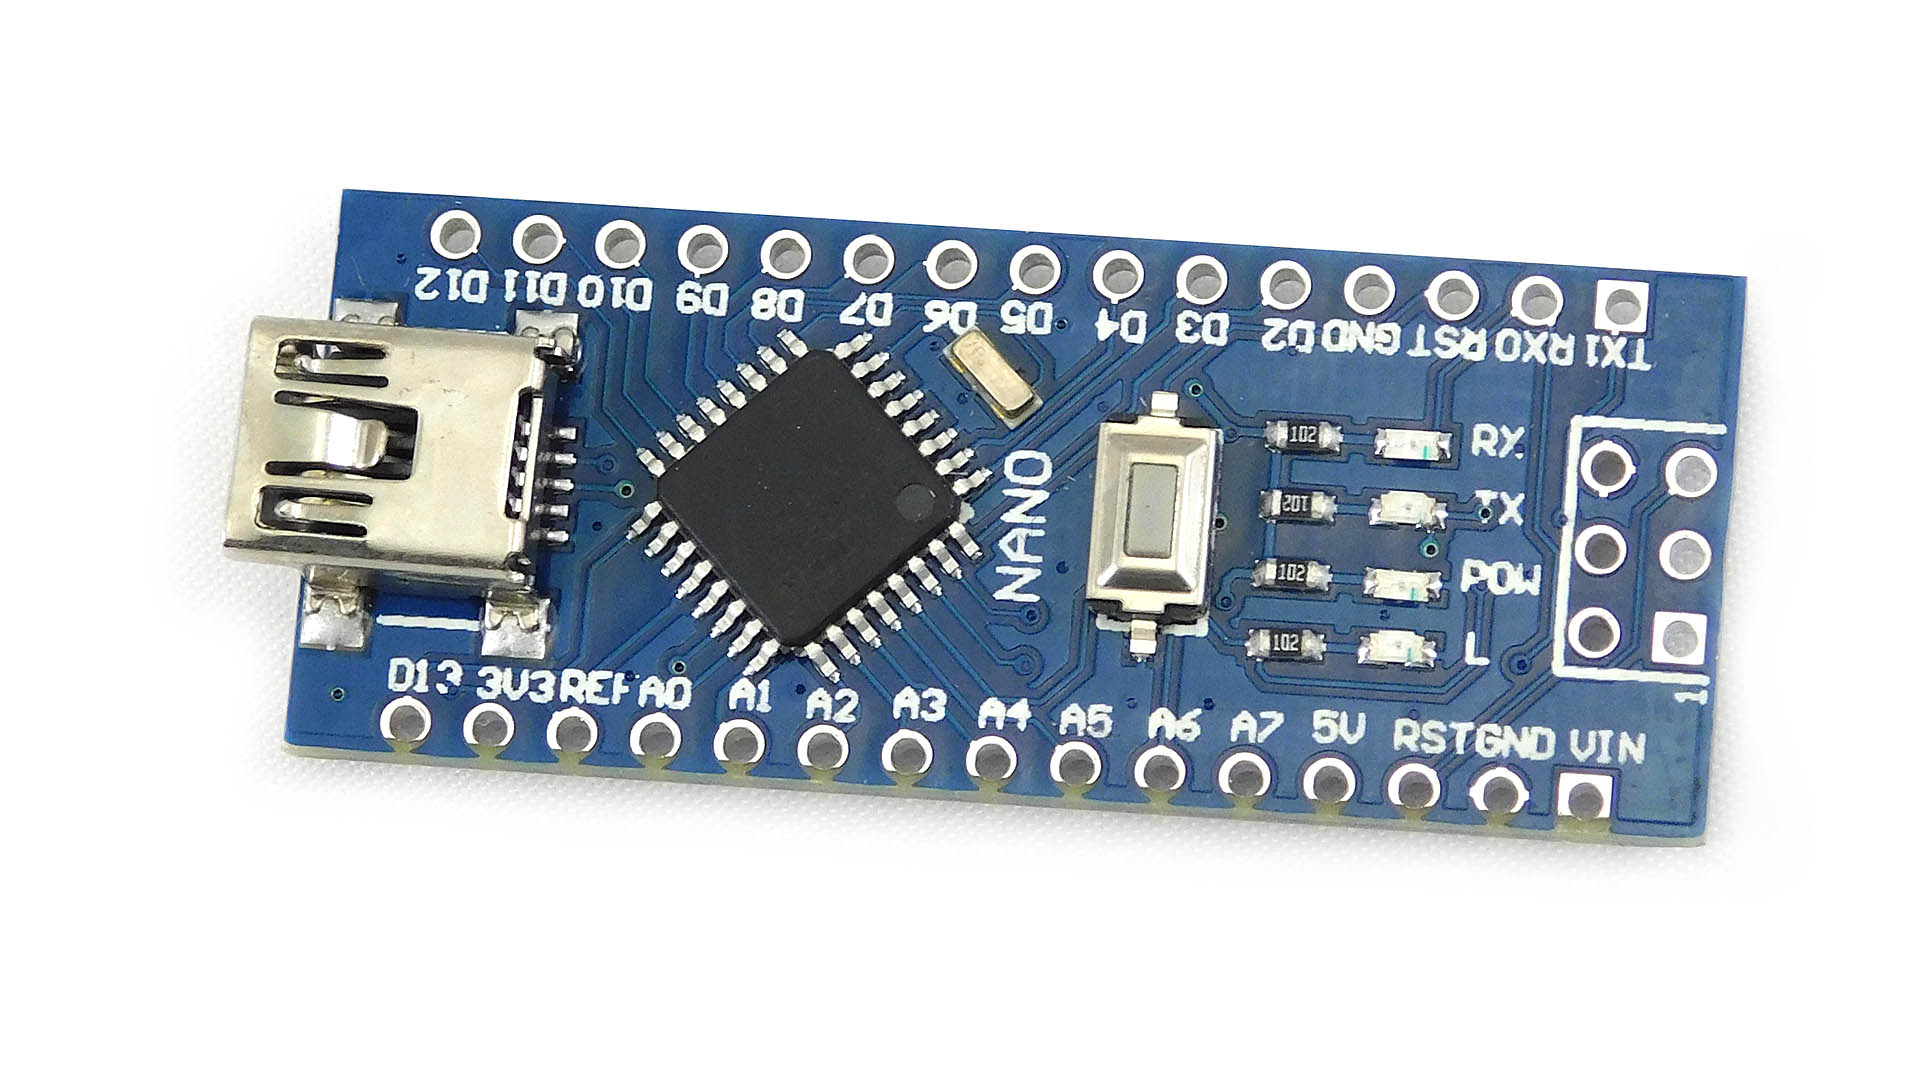
\includegraphics[scale=0.15]{Chapter 3/image chapter 3/nano.jpg}
	\caption[Arduino nano CH340]{Arduino nano CH340}
	\label{hinh31}
\end{figure}
Mạch Arduino Nano CH340 có kích thước nhỏ gọn, có thiết kế và chuẩn chân giao tiếp tương đương với Arduino Nano chính hãng, tuy nhiên mạch sử dụng chip nạp chương trình và giao tiếp UART CH340 giá rẻ để tiết kiệm chi phí.\\
\indent Arduino Nano là phiên bản nhỏ gọn của Arduino Uno R3 sử dụng MCU ATmega328P-AU dán, vì cùng MCU nên mọi tính năng hay chương trình chạy trên Arduino Uno đều có thể sử dụng trên Arduino Nano, một ưu điểm của Arduino Nano là vì sử dụng phiên bản IC dán nên sẽ có thêm 2 chân Analog A6, A7 so với Arduino Uno.\\
\begin{figure}[H]
	\centering
	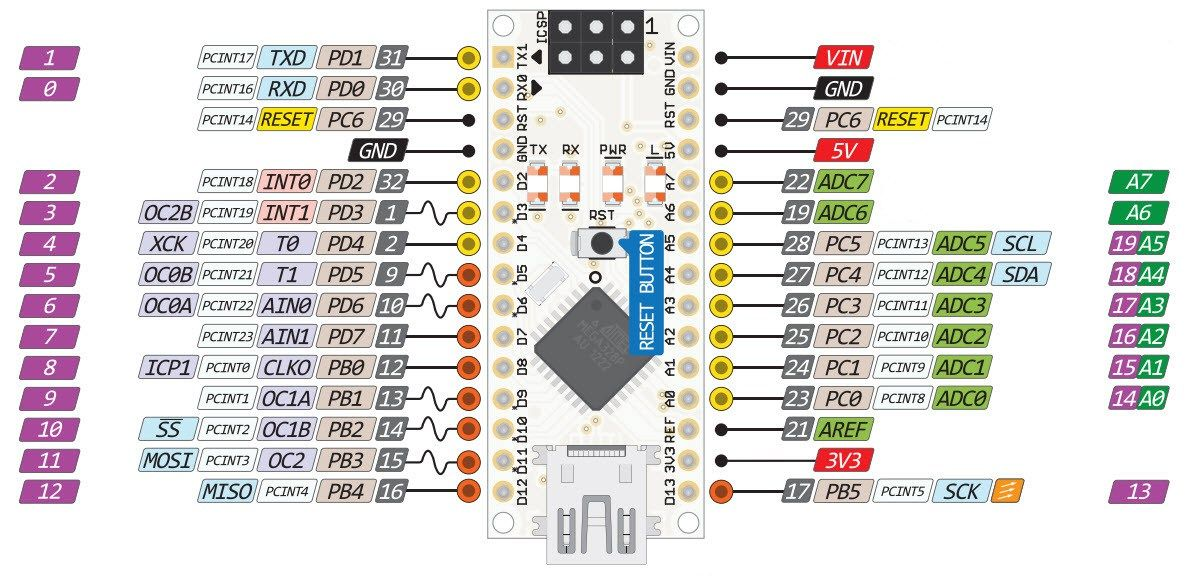
\includegraphics[scale=.7]{Chapter 3/image chapter 3/sodoNano.png}
	\caption[Sơ đồ chân của Arduino nano CH340]{Sơ đồ chân của Arduino nano CH340}
	\label{hinh32}
\end{figure}
\indent \textbf{Thông số kỹ thuật:}\\
\begin{itemize}
	\item Thiết kế theo đúng chuẩn chân, kích thước của Arduino Nano chính hãng.
	\item IC chính: ATmega328P-AU.
	\item IC nạp và giao tiếp UART: CH340.
	\item Điện áp cấp: 5VDC cổng USB hoặc 6-9VDC chân Raw.
	\item Mức điện áp giao tiếp GPIO: TTL 5VDC.
	\item Dòng GPIO: 40mA.
	\item Số chân Digital: 14 chân, trong đó có 6 chân PWM.
	\item Số chân Analog: 8 chân (hơn Arduino Uno 2 chân).
	\item Flash Memory: 32KB (2KB Bootloader).
	\item SRAM: 2KB
	\item EEPROM: 1KB
	\item Clock Speed: 16Mhz.
	\item Tích hợp Led báo nguồn, led chân D13, LED RX, TX.
	\item Tích hợp IC chuyển điện áp 5V LM1117.
	\item Kích thước: 18.542 x 43.18mm
\end{itemize}
\subsection{RASPBERRY PI 3 MODEL B+}
\begin{figure}[H]
	\centering
	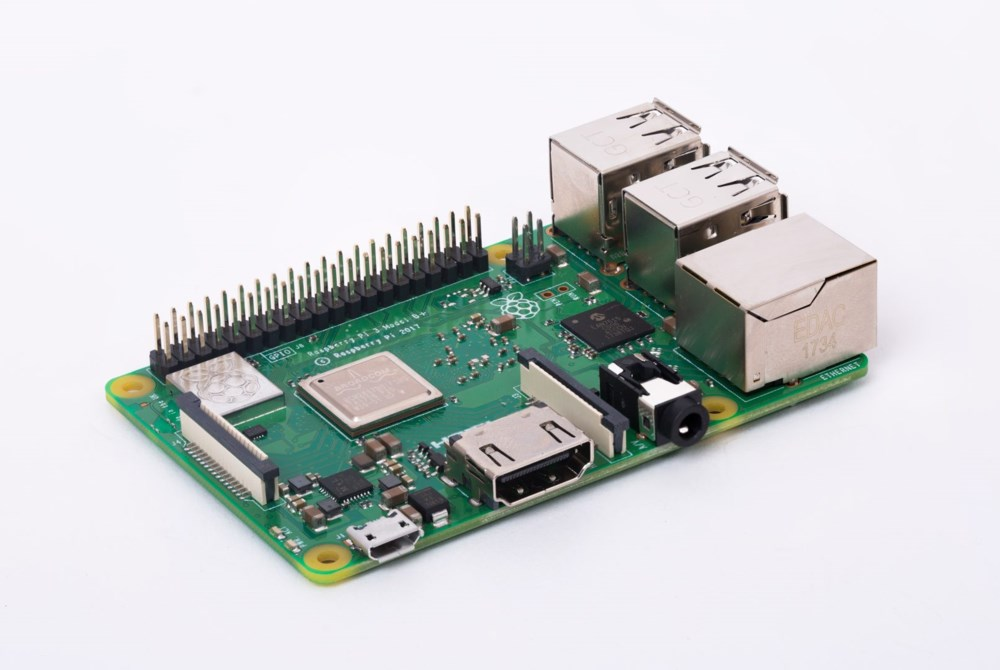
\includegraphics[scale=.5]{Chapter 3/image chapter 3/rasp3.jpg}
	\caption[Raspberry Pi 3 Model B+ ]{Raspberry Pi 3 Model B+}
	\label{hinh33}
\end{figure}
Raspberry Pi 3 Model B+ là một phiên bản nâng cấp của Raspberry Pi 3 Model B đã từng ra mắt cách đây hơn 2 năm. Trước kia, thường khoảng 1 năm thì Raspberry Pi sẽ được nâng cấp 1 lần nhưng từ phiên bản 3 thì Raspberry Pi đã làm điều này chậm hơn một chút dù doanh số bán lên tới 14 triệu máy.\\
\indent Với thế hệ Raspberry Pi 3 mới nhất và mạnh nhất hiện nay trong dòng Raspberry Pi, bản nâng cấp vừa ra mắt hôm nay chủ yếu mang đến tốc độ nhanh hơn về mọi mặt.\\
\indent Cụ thể, điểm nâng cấp chính của Raspberry Pi 3 Model B+ là vi xử lý và kết nối mạng. Model B+ dùng vi xử lý Broadcom BCM2837B0 4 nhân 1.4GHz (cao hơn so với BCM2837 1.2GHz trên Pi 3 Model B).\\
\indent Với các công việc đòi hỏi tốc độ mạng nhanh, Pi 3 Model B+ có thể đáp ứng với kết nối Wi-Fi 2 băng tần 2.4GHz và 5GHz (dual band), Ethernet gigabit (qua cổng USB 2.0) tốc độ lên đến 300Mbps, gấp 3 lần so với Pi 3 Model B. Thiết bị cũng hỗ trợ Bluetooth 4.2 và Bluetooth LE giúp kết nối tốt hơn với các thiết bị thông minh khác.\\
\indent Cuối cùng, Model B+ còn có Power over Ethernet (PoE) giúp cung cấp nguồn điện cho thiết bị thông qua dây cắm Ethernet nhưng phải thông qua một HAT mở rộng.\\
\indent Ngoài những nâng cấp trên thì ngoại hình và kích thước Model B+ vẫn y hệt Model B nên hoàn toàn tương thích với mọi case và phụ kiện trước đây dành cho Model B. Cấu hình chi tiết Raspberry Pi 3 Model B+:
\begin{itemize}
	\item SoC: Broadcom BCM2837B0, Cortex-A53 (ARMv8) 64-bit SoC @ 1,4 GHz
	\item RAM: 1 GB LPDDR2 SDRAM
	\item Wi-Fi b/g/n/ac
	\item Bluetooth 4.2, BLE
	\item Gigabit Ethernet over USB 2.0 (maximum throughput 300 Mbps)
	\item 40-pin GPIO
	\item HDMI
	\item 4 x cổng USB 2.0
	\item Khe cắm thẻ Micro SD
	\item Hỗ trợ Power-over-Ethernet (PoE)
	\item Cải thiện PXE network và USB mass-storage booting
	\item Tản nhiệt tốt hơn Model B
\end{itemize}
\begin{figure}[H]
	\centering
	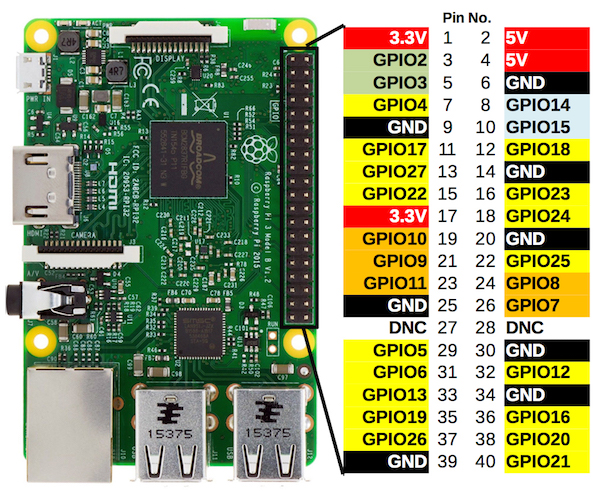
\includegraphics[scale=.5]{Chapter 3/image chapter 3/raspGPIO.jpg}
	\caption[Sơ đồ các chân GPIO của Raspberry Pi 3 Model B+]{Sơ đồ các chân GPIO của Raspberry Pi 3 Model B+}
	\label{hinh34}
\end{figure}
\subsection{MODULE RF UART E32-TTL-100}
\begin{figure}[H]
	\centering
	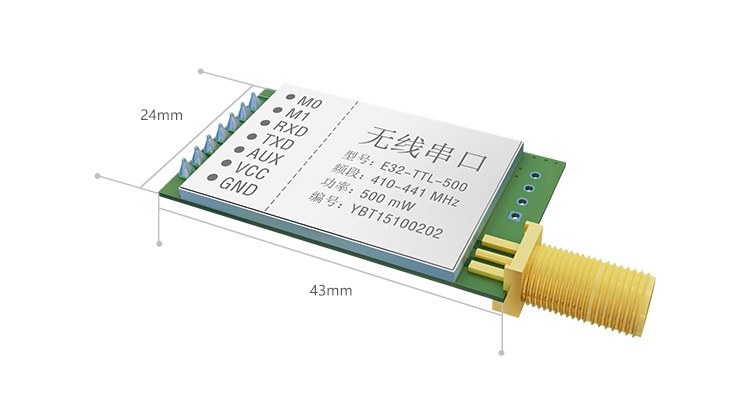
\includegraphics[scale=.4]{Chapter 2/image chapter 2/E32.jpg}
	\caption[Module RF UART E32-TTL-100]{Module RF UART E32-TTL-100}
	\label{hinh35}
\end{figure}
\begin{figure}[H]
	\centering
	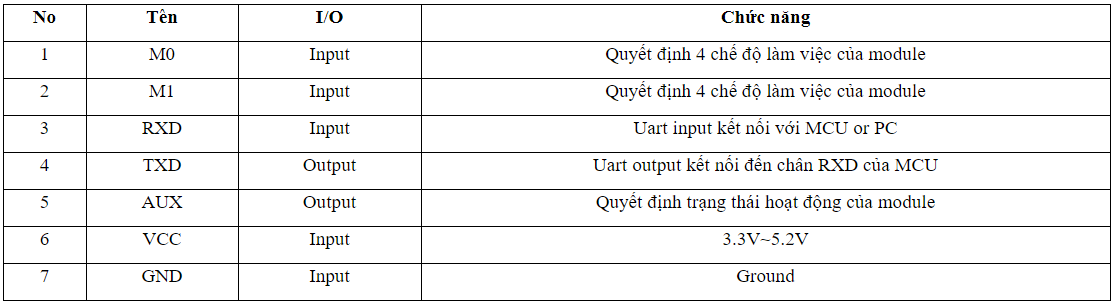
\includegraphics[scale=.5]{Chapter 2/image chapter 2/sodochanvachucnangE32.png}
	\caption[Sơ đồ chân và chức năng của module LoRa E32]{Sơ đồ chân và chức năng của module LoRa E32}
	\label{hinh36}
\end{figure}
Mạch thu phát RF UART Lora SX1278 433Mhz 3000m sử dụng chip SX1278 của nhà sản xuất SEMTECH chuẩn giao tiếp LORA (Long Range), chuẩn LORA mang đến hai yếu tố quan trọng là tiết kiệm năng lượng và khoảng cách phát siêu xa ( Ultimate long range wireless solution), ngoài ra nó còn có khả năng cấu hình để tạo thành mạng nên hiện tại được phát triển và sử dụng rất nhiều trong các nghiên cứu về IoT.\\
\indent Mạch thu phát RF UART Lora SX1278 433Mhz 3000m được tích hợp phần chuyển đổi giao tiếp SPI của SX1278 sang UART giúp việc giao tiếp và sử dụng rất dễ dàng, chỉ cần kết nối với Software của hãng để cấu hình địa chỉ , tốc độ và công suất truyền là có thể sử dụng.\\
\indent \textbf{Thông số kỹ thuật:}
\begin{itemize}
	\item Model: E32-TTL-100 RF
	\item Điện áp hoạt đông: 2.3 - 5.5 VDC
	\item Điện áp giao tiếp: TTL-3.3V
	\item Giao tiếp UART Data bits 8, Stop bits 1, Parity none, tốc độ từ 1200 - 115200.
	\item Tần số: 410 - 441Mhz
	\item Công suất: 20dbm (100mW)
	\item Khoảng cách truyền tối đa trong điều kiện lý tưởng: 3000m
	\item Tốc độ truyền: 0.3 - 19.2 Kbps ( mặc định 2.4 Kbps)
	\item 512bytes bộ đệm
	\item Hỗ trợ 65536 địa chỉ cấu hình.
	\item Kích thước: 21x36mm.
\end{itemize}
\begin{figure}[H]
	\centering
	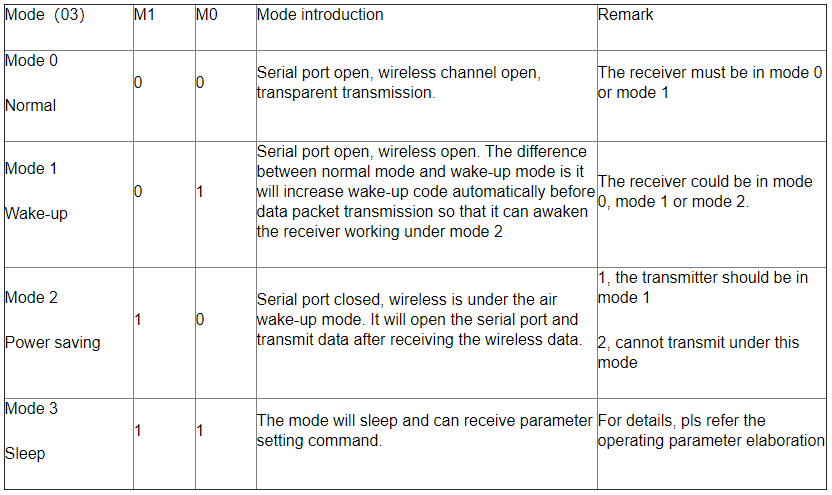
\includegraphics[scale=.5]{Chapter 2/image chapter 2/workmodeE32.png}
	\caption[Chế độ làm việc của module LoRa E32]{Chế độ làm việc của module LoRa E32}
	\label{hinh37}
\end{figure}

\indent Các bước cấu hình cho module E32 LoRa:
\begin{itemize}
	\item Để tùy chỉnh các thông số thu phát: Kênh, Địa chỉ, Tốc độ, Công suất,… chúng ta cần sử dụng module chuyển đổi USB-UART Lora CP2102 kết nối với máy tính.
	\item Kết nối với máy tính, tải và cài đặt Driver CP210x.
	\item Sau đó sử dụng phần mềm Wireless Module Setting để tiến hành tùy chỉnh.
\end{itemize}
\begin{figure}[H]
	\centering
	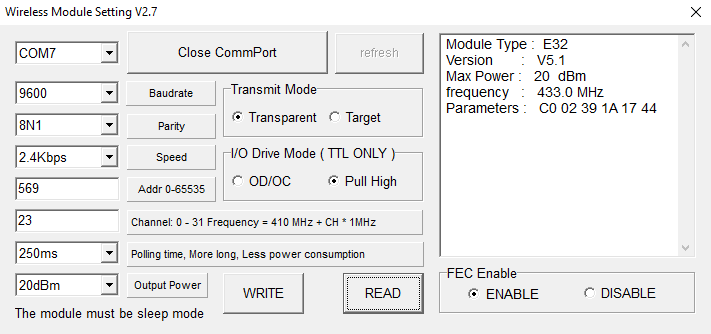
\includegraphics[scale=.5]{Chapter 2/image chapter 2/configLoRa.png}
	\caption[Phần mềm cấu hình module LoRa E32]{Phần mềm cấu hình module LoRa E32}
\end{figure}

\indent \textbf{Lưu ý:} Để các module có thể giao tiếp được với nhau, thì các thông số tùy chỉnh như: kênh truyền, địa chỉ,… cần \textbf{phải giống nhau}.
\subsection{DHT22 TEMPERATURE AND HUMIDITY SENSOR}
\begin{figure}[H]
	\centering
	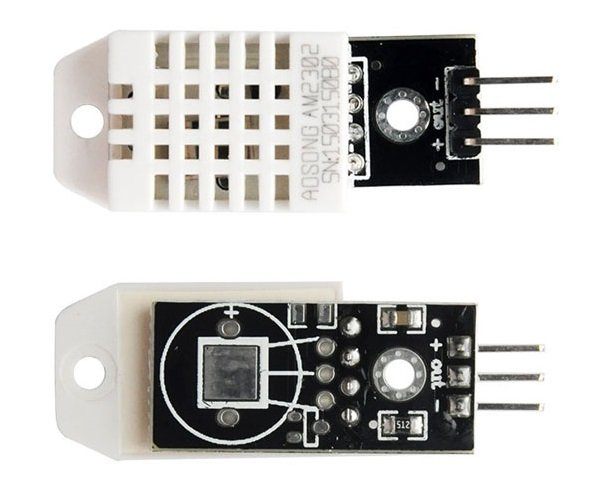
\includegraphics[scale=.5]{Chapter 3/image chapter 3/DHT22.jpg}
	\caption[Module DHT22]{Module DHT22}
	\label{hinh38}
\end{figure}
Cảm biến độ ẩm, nhiệt độ DHT22 Temperature Humidity Sensor ra chân là phiên bản ra chuẩn chân cắm thông dụng 2.54mm hàn sẵn trên mặt in với trở kéo dễ dàng sử dụng, ứng ụng đo độ ẩm, nhiệt độ môi trường với độ chính xác cao, cảm biến có chất lượng tốt, độ bền và độ ổn định cao.\\
\indent \textbf{Thông số kỹ thuật:}
\begin{itemize}
	\item Nguồn sử dụng: 3~5 VDC.
	\item Dòng sử dụng: 2.5mA max (khi truyền dữ liệu).
	\item Đo tốt ở độ ẩm 0100\% RH với sai số 2-5\%.
	\item Đo tốt ở nhiệt độ -40 to 80°C sai số ±0.5°C.
	\item Tần số lấy mẫu tối đa 0.5Hz (2 giây 1 lần)
	\item Kích thước 27mm x 59mm x 13.5mm (1.05" x 2.32" x 0.53")
	\item Chân tín hiệu: 5VDC(+) | OUT | GND (-) (chân out nối trực tiếp với chân giao tiếp của VĐK không cần trở kéo vì đã có sẵn trên mạch).
\end{itemize}
\subsection{MODULE 2 RELAY OPTO 5VDC}
\begin{figure}[H]
	\centering
	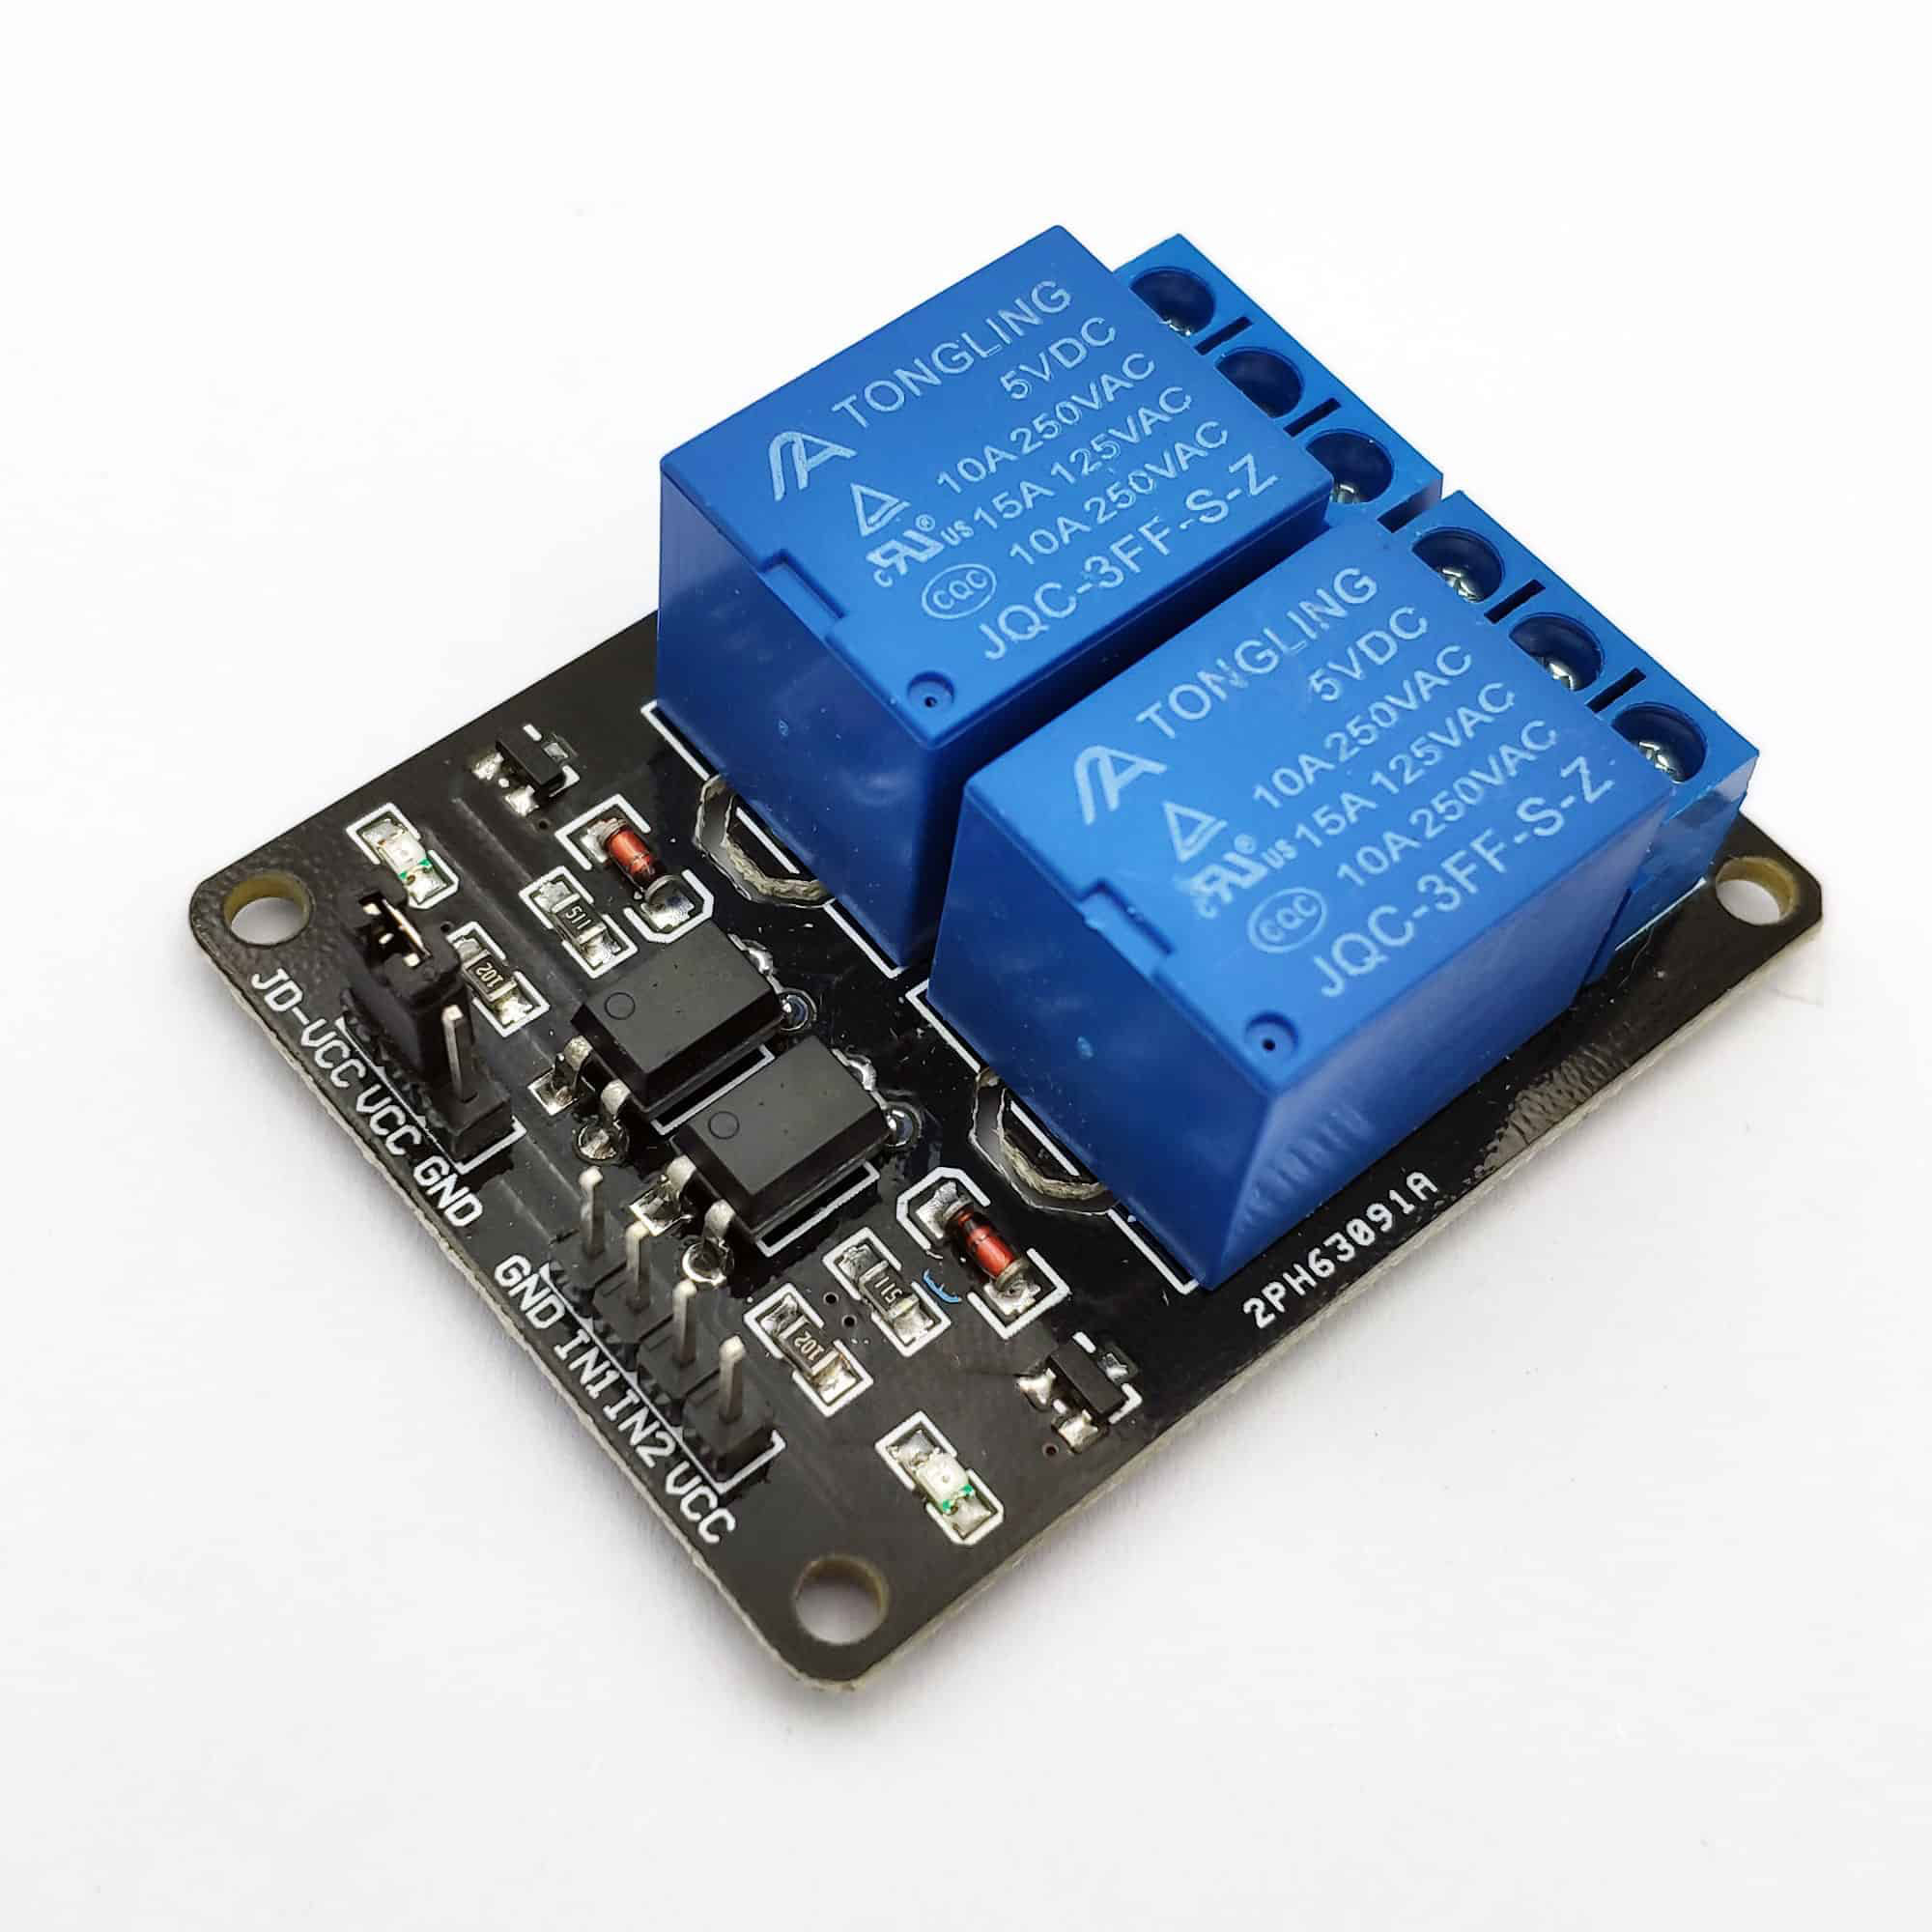
\includegraphics[scale=.1]{Chapter 3/image chapter 3/2relay.jpg}
	\caption[Module 2 relay opto 5VDC]{Module 2 relay opto 5VDC}
	\label{hinh39}
\end{figure}
Mạch 2 Relay Opto cách ly 5VDC thích hợp với các ứng dụng đóng ngắt tải AC hoặc DC, mạch có thiết kế nhỏ gọn, tích hợp opto và transistor cách ly, kích đóng bằng mức thấp (0VDC) phù hợp với mọi loại MCU và thiết kế có thể sử dụng nguồn ngoài giúp cho việc sử dụng trở nên thật linh động và dễ dàng.\\
\indent \textbf{Thông số kỹ thuật:}
\begin{itemize}
	\item Điện áp sử dụng: 5VDC
	\item Tín hiệu kích: TTL 3.3~5VDC, mức thấp Low Relay đóng, mức cao High Relay ngắt.
	\item Mỗi Relay tiêu thụ dòng khoảng 80mA.
	\item Điện thế đóng ngắt tối đa: AC250V ~ 10A hoặc DC30V ~ 10A (Để an toàn nên dùng cho tải có công suất <100W).
	\item Tích hợp Opto cách ly, Diod chống nhiễu và đèn báo tín hiệu kích.
	\item Kích thước: 39 x 51 x 20mm
\end{itemize}
\subsection{CẢM BIẾN ĐỘ ĐỤC NƯỚC (DFROBOT)}
\begin{figure}[H]
	\centering
	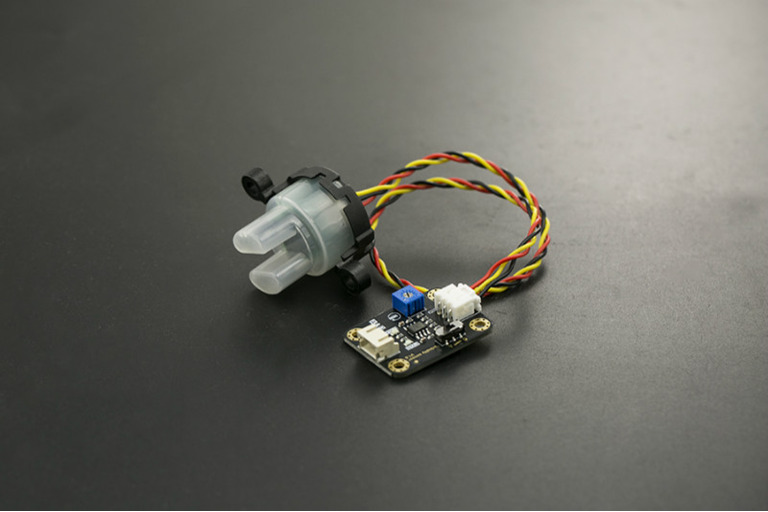
\includegraphics[scale=.3]{Chapter 3/image chapter 3/TurbiSensor.jpg}
	\caption[Cảm biến độ đục nước (DFROBOT)]{Cảm biến độ đục nước (DFROBOT)}
\end{figure}
Độ đục là một trong những tiêu chí dùng để kiểm tra chất lượng nước, nó thể hiện bằng lượng hạt tồn tại trong nước, lượng hạt càng tăng thì mức độ đục của nước càng tăng\\
\indent Vì thế kiểm tra độ đục của nước là cần thiết.\\
\indent Cảm biến đo độ đục chất lỏng giúp chúng ta có thể đo mức độ đục của chất lỏng\\
\indent Cảm biến đo độ đục chất lỏng hoạt động dựa vào nguyên lý quang học, nó có thể phát hiện các hạt lơ lửng trong nước.\\
\indent \textbf{Ứng dụng}\\
\indent Cảm biến đo độ đục chất lỏng được ứng dụng trong bài toán như:
\begin{itemize}
	\item Đo chất lượng nước ở sông, suối, hay trong các đường ống nước
	\item Đo chất lượng nước thải
	\item Dùng trong nghiên cứu, thí nghiệm
\end{itemize}

\indent \textbf{Thông số kỹ thuật}
\begin{itemize}
	\item Điện áp hoạt động: 5V
	\item Dòng điện làm việc: 40mA (Max)
	\item Thời gian đáp ứng: < 500ms
	\item Điện trở cách điện: 100M(Min)
	\item Đầu ra Analog 0 ~ 4.5V
	\item Đầu ra Digital: High/Low (Có thể điều chỉnh giá trị ngưỡng bằng biến trở)
	\item Nhiệt độ hoạt động: 5*C ~ 90*C
	\item Nhiệt độ dự trữ: -10*C ~ 90*C
	\item Kích thước: 38mm*28mm*10mm
	\item Trọng lượng: 30g
\end{itemize}

\indent \textbf{Sơ đồ các chân}
\begin{figure}[H]
	\centering
	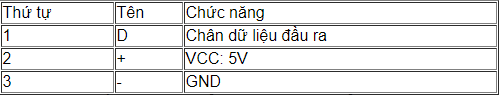
\includegraphics[scale=1]{Chapter 3/image chapter 3/sodoTurbi.PNG}
	\caption[Sơ đồ và chức năng của các chân cảm biến]{Sơ đồ và chức năng của các chân cảm biến}
\end{figure}
\indent Chân dữ liệu đầu ra "D" có thể chọn là chân ra kiểu "Digital" hoặc "Analog" thông qua công tắc gạt trên cảm biến
\subsection{CẢM BIẾN pH (Atlas Scientific)}
\begin{figure}[H]
	\centering
	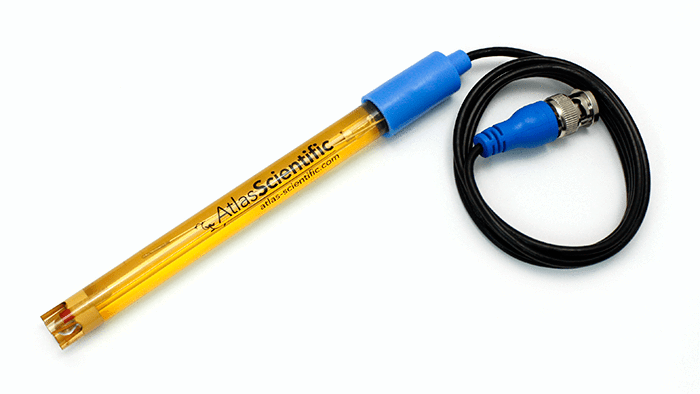
\includegraphics[scale=.4]{Chapter 3/image chapter 3/pHSensor.png}
	\caption[Cảm biến pH]{Cảm biến pH}
\end{figure}
Bộ cảm biến PH Atlas Scientific là một mạch cảm biến pH nhúng thế hệ thứ 6. Mạch pH lớp EZO này, mang lại độ ổn định và độ chính xác cao nhất.\\
\indent Với cấu hình phù hợp, mạch pH lớp EZO có thể đáp ứng hoặc vượt quá độ chính xác và độ chính xác so với hầu hết các máy đo pH trong phòng thí nghiệm. Mạch pH pH-EZO, có thể hoạt động với bất kỳ đầu dò/cảm biến/điện cực pH nào có sẵn.\\
\indent \textbf{Thông số kỹ thuật:}
\begin{itemize}
	\item Tầm đo: 0-14 (sai số Na + ở> 12,3 pH)
	\item Nhiệt độ hoạt động: 1*C - 99*C
	\item Áp suất tối đa: 690 kPa (100PSI)
	\item Độ sâu tối đa: 60M (197 ft)
	\item Chiều dài cáp: 1 mét
	\item Trọng lượng: 49 gram
	\item Tốc độ phản hồi: 95\% trong 1 giây
	\item Điểm đẳng tích: pH 7,00 (0 mV)
	\item Kích thước: 12mm X 150mm (1/2 "X 6")
	\item Đầu nối BNC 
\end{itemize}
\subsection{CẢM BIẾN ORP (Atlas Scientific)}
\begin{figure}[H]
	\centering
	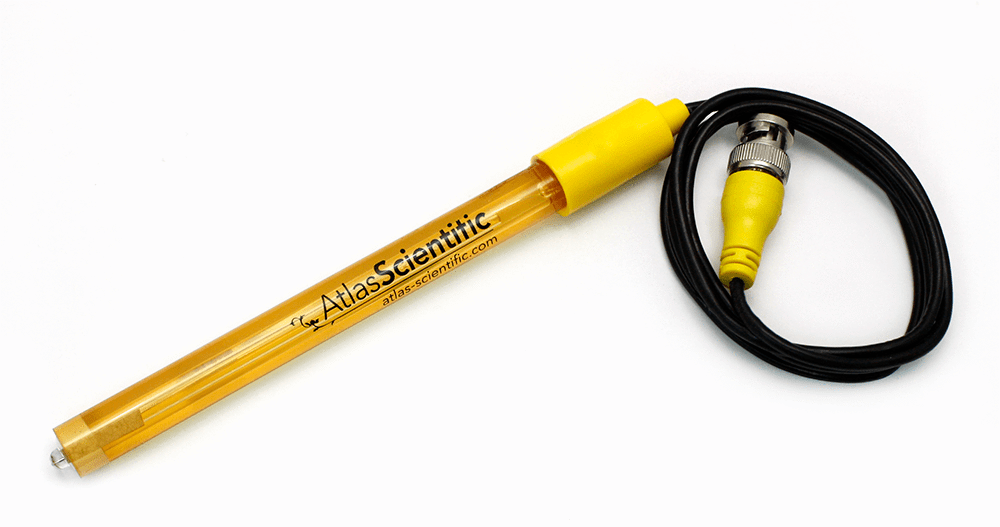
\includegraphics[scale=.3]{Chapter 3/image chapter 3/ORPSensor.png}
	\caption[Cảm biến ORP]{Cảm biến ORP}
\end{figure}
ORP Probe hoàn hảo cho thiết bị đo ORP cho hệ thống thủy canh, lấy mẫu đất, sử dụng trong phòng thí nghiệm tiêu chuẩn, sử dụng ngoài đồng ruộng, an toàn thực phẩm, nước ion thấp và siêu tinh khiết, giữ cá, chất khử mạnh. Đầu dò ORP này có thể được ngâm hoàn toàn trong nước ngọt hoặc nước muối, cho đến đầu nối BNC vô thời hạn. Mạch EZO ORP mang lại độ ổn định và độ chính xác cao nhất. Với cấu hình phù hợp, mạch EZO ORP, có thể đáp ứng hoặc vượt quá độ chính xác và độ chính xác so với các máy đo ORP để bàn trong phòng thí nghiệm.
\begin{itemize}
	\item ORP Calibration Solution được thiết kế để hiệu chuẩn và kiểm tra chính xác thiết bị cho đầu dò ORP. Để sử dụng giải pháp này, Đặt đầu dò ORP của bạn vào dung dịch này, để yên 1-2 phút. Máy đo của bạn sau đó sẽ đọc 225mV nếu được hiệu chuẩn chính xác.
	\item Mạch EZO ORP mang lại độ ổn định và độ chính xác cao nhất. Với cấu hình phù hợp, mạch EZO ORP có thể đáp ứng hoặc vượt quá độ chính xác và độ chính xác được tìm thấy trong các máy đo ORP cấp phòng thí nghiệm để bàn. Mạch ORP có thể hoạt động với bất kỳ đầu dò/cảm biến/điện cực ORP nào có sẵn.
	\item Bộ cảm biến ORP / REDOX có khả năng đọc phụ thuộc nhiệt độ hoặc độc lập với nhiệt độ cũng như chế độ đọc đơn hoặc đọc liên tục. Giao thức hiệu chuẩn linh hoạt hỗ trợ hiệu chuẩn một điểm đến bất kỳ giá trị nào. Số đọc ORP phạm vi rộng từ -1019,9 đến +1019,9. Số đọc ORP chính xác đến hàng trăm (+/-1mV).
\end{itemize}

\indent Đầu dò ORP này có thể được ngâm hoàn toàn trong nước ngọt hoặc nước muối, cho đến đầu nối BNC vô thời hạn. Đầu dò ORP là một thiết bị thụ động phát hiện dòng điện được tạo ra từ thế oxy hóa-khử của nước.

\section*{CHƯƠNG 4: KẾT QUẢ THỰC HIỆN}
\addcontentsline{toc}{section}{\numberline {} CHƯƠNG 4: KẾT QUẢ THỰC HIỆN}
\setcounter{section}{4}
\setcounter{figure}{0}
\setcounter{subsection}{0}
\subsection{KẾT QUẢ THI CÔNG PHẦN CỨNG}
Mô hình phần cứng của đồ án này bao gồm, 2 node Arduino giao tiếp với gateway Raspberry thông qua mạng LoRa để truyền các dữ liệu cảm biến như nhiệt độ, độ ẩm, ... ở node ao tôm và node vườn thanh long. Đồng thời nhận lệnh điều khiển từ gateway để bật tắt 2 relay "Máy bơm nước" và "Đèn" ở node vườn thanh long. Dưới đây là ảnh minh hoạ cho mô hình truyền/nhận của phần cứng:
\begin{figure}[H]
	\centering
	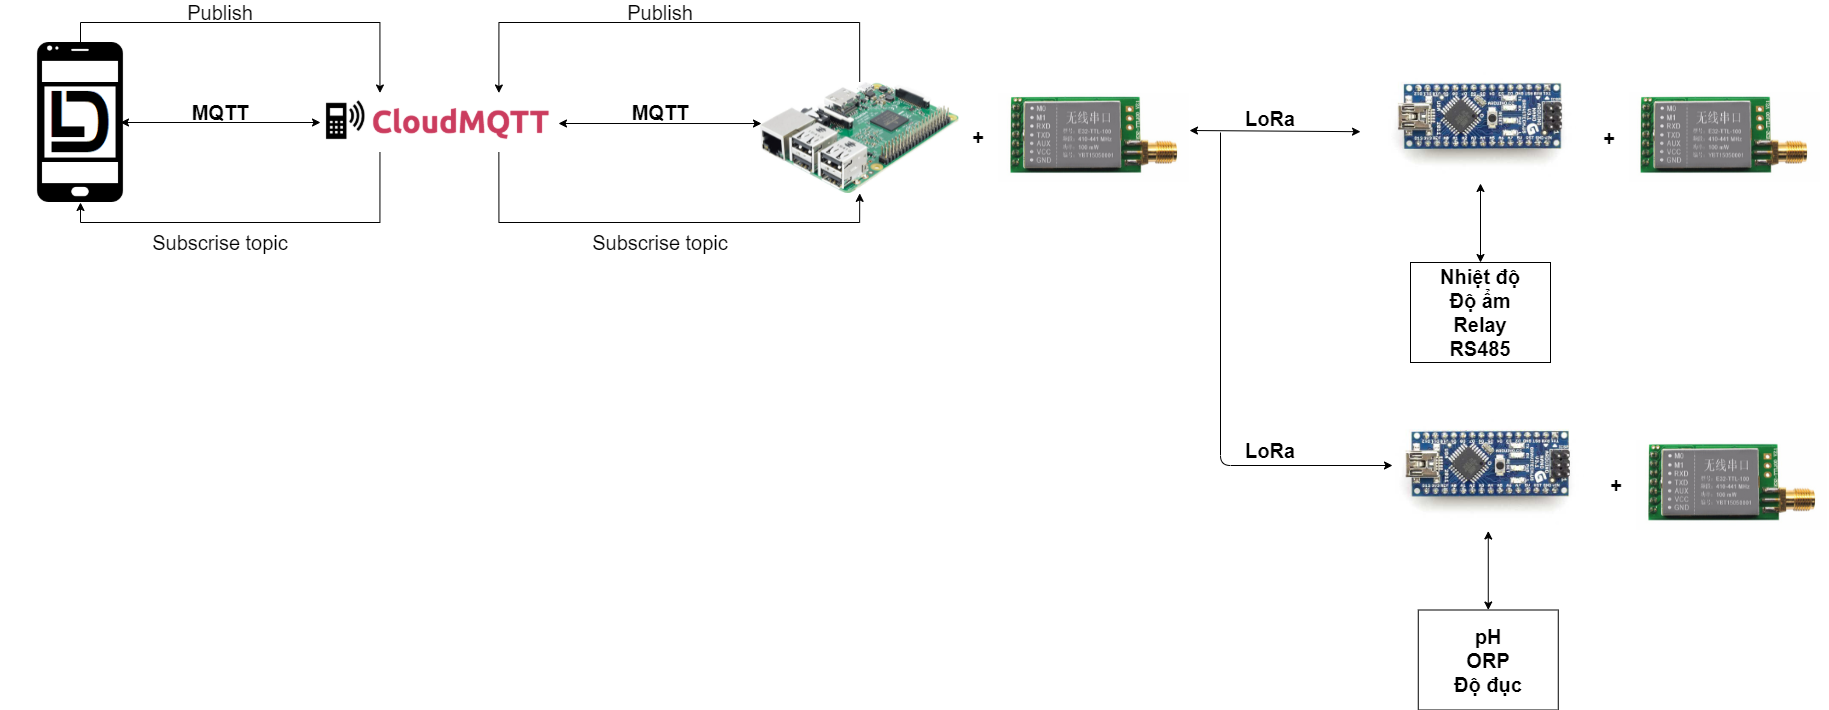
\includegraphics[scale=0.2]{Chapter 4/image chapter 4/sodoDCLV.png}
	\caption[Sơ đồ các giao tiếp phần cứng]{Sơ đồ các giao tiếp phần cứng}
	\label{hinh41}
\end{figure}
\subsubsection{Hình ảnh phần cứng thực tế của node đặt ở vườn thanh long}
\indent Do vẫn còn phát triển thêm: gắn thêm cảm biến, thay thế 1 số linh kiện cho phù hợp, ... Nên em vẫn còn dùng bread board để cắm mạch cho tiện việc nghiên cứu. Trong tương lai, khi tiến hành phát triển lên Luận văn Tốt nghiệp, em sẽ đưa mạch này lên PCB.
\begin{figure}[H]
	\centering
	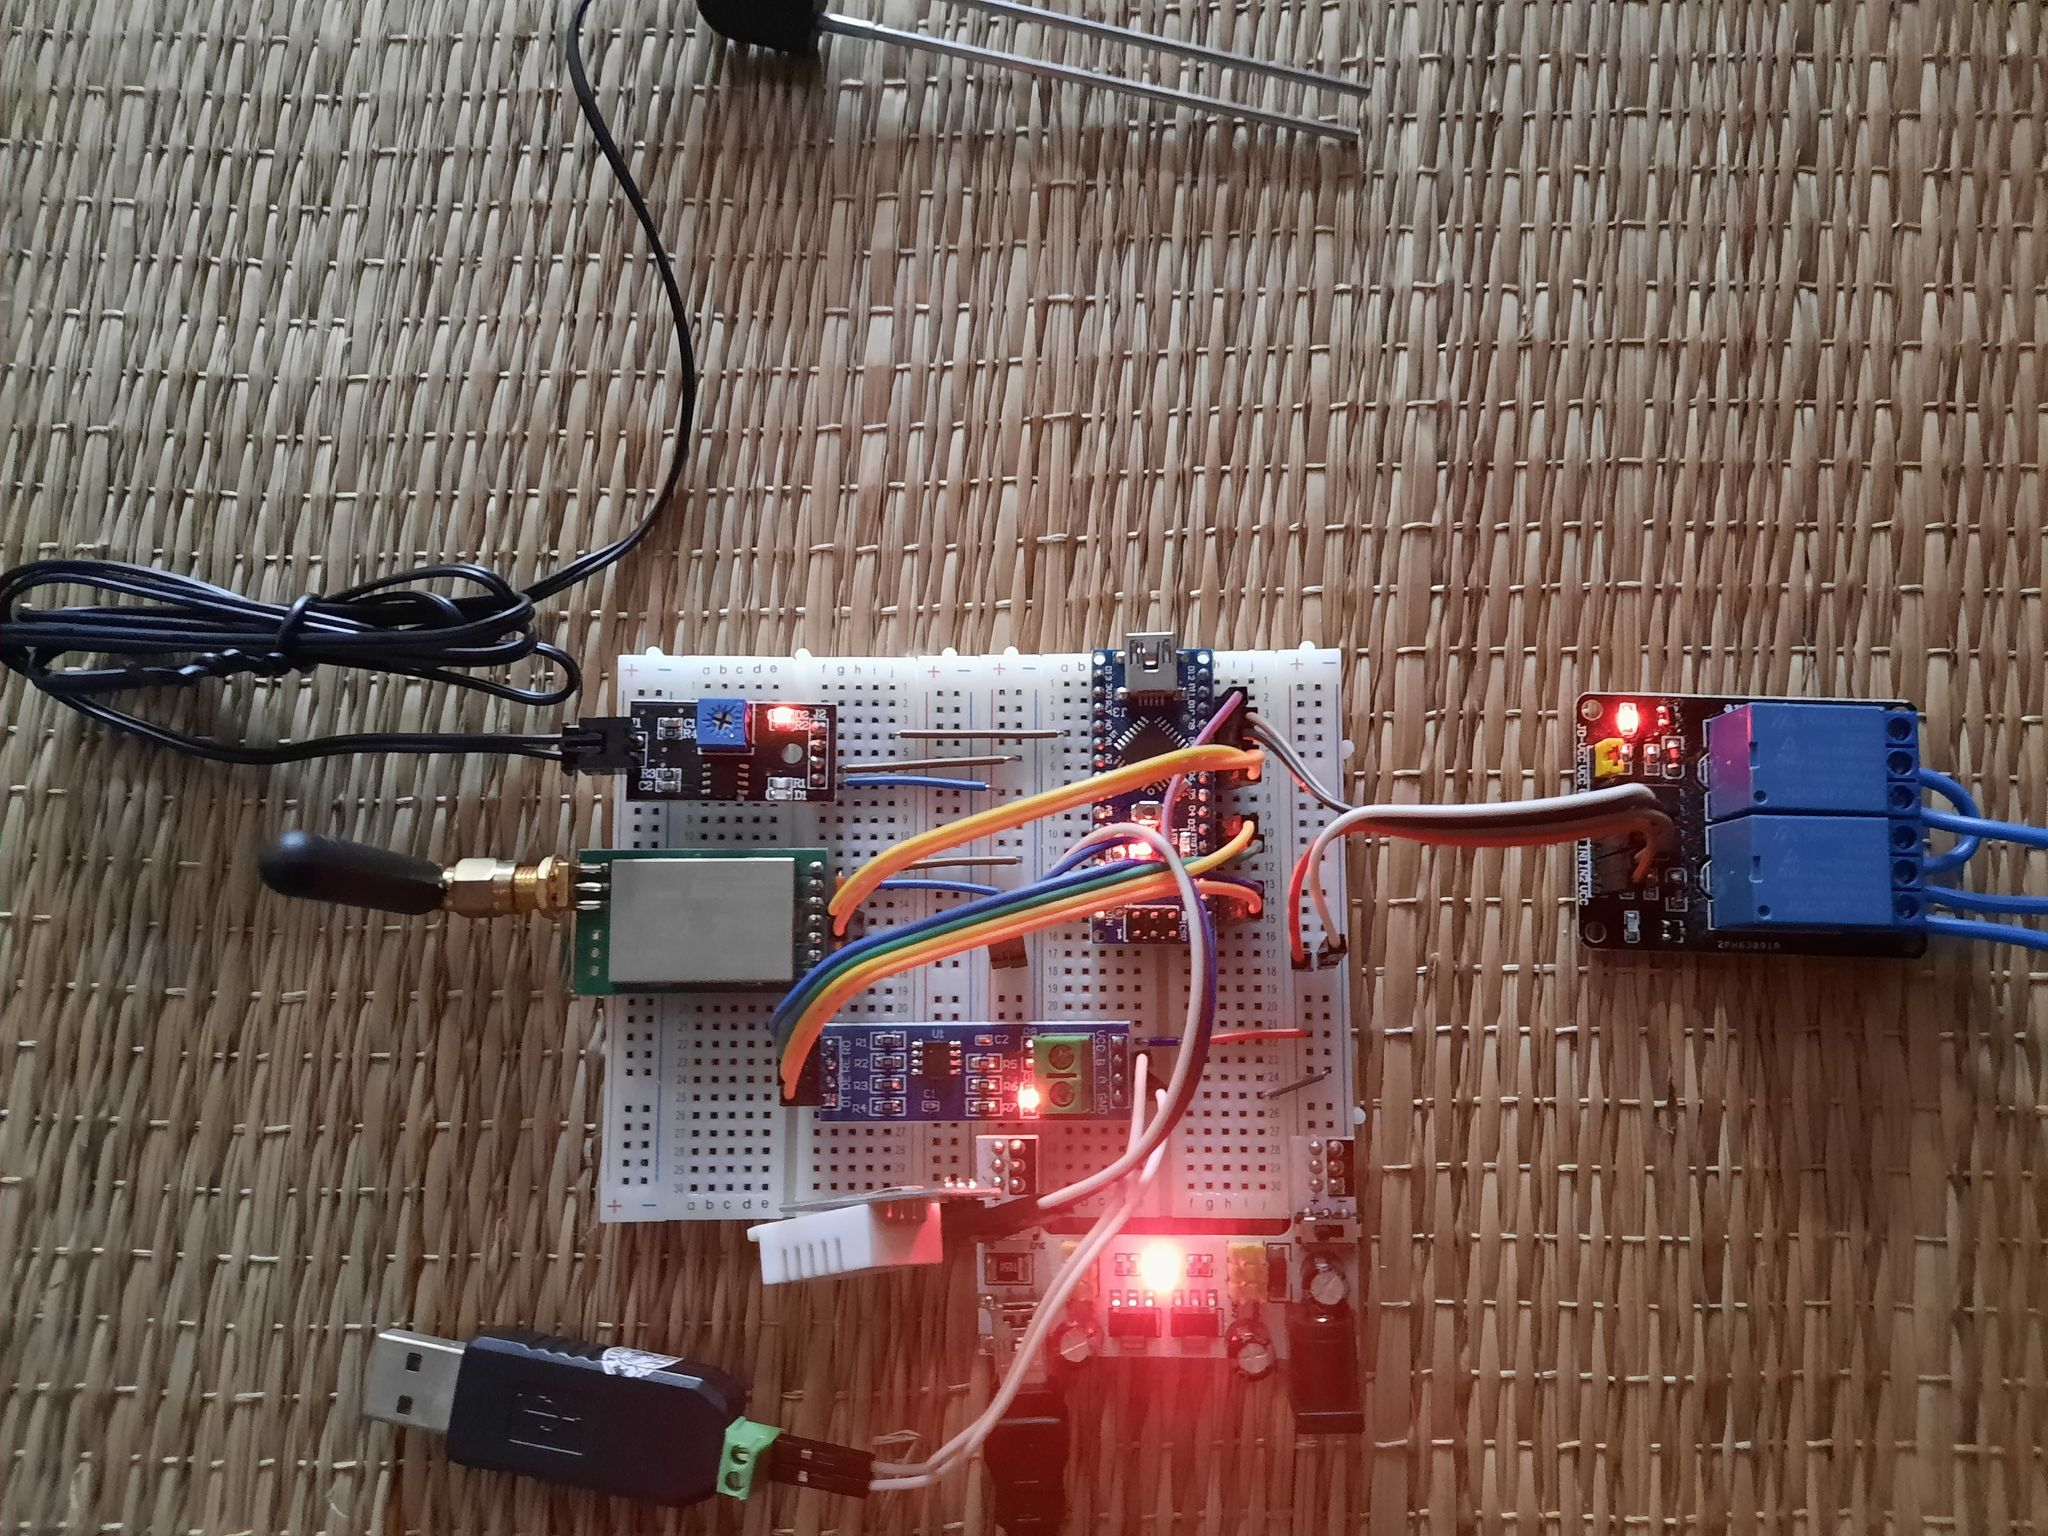
\includegraphics[scale=0.1]{Chapter 4/image chapter 4/phancung.jpg}
	\caption[Phần cứng node vườn thanh long thực tế]{Phần cứng node vườn thanh long thực tế}
	\label{hinh42}
\end{figure}
\subsubsection{Hình ảnh phần cứng thực tế của node đặt ở ao tôm}
\indent Node đặt ở ao tôm, được em đầu tư đóng hộp để bảo vệ các linh kiện điện tử bên trong, cũng như hạn chế được các tác động của môi trường, thời tiết bên ngoài tác động, ảnh hưởng đến độ bền và khả năng hoạt động của hệ thống bên trong.
\begin{figure}[H]
	\centering
	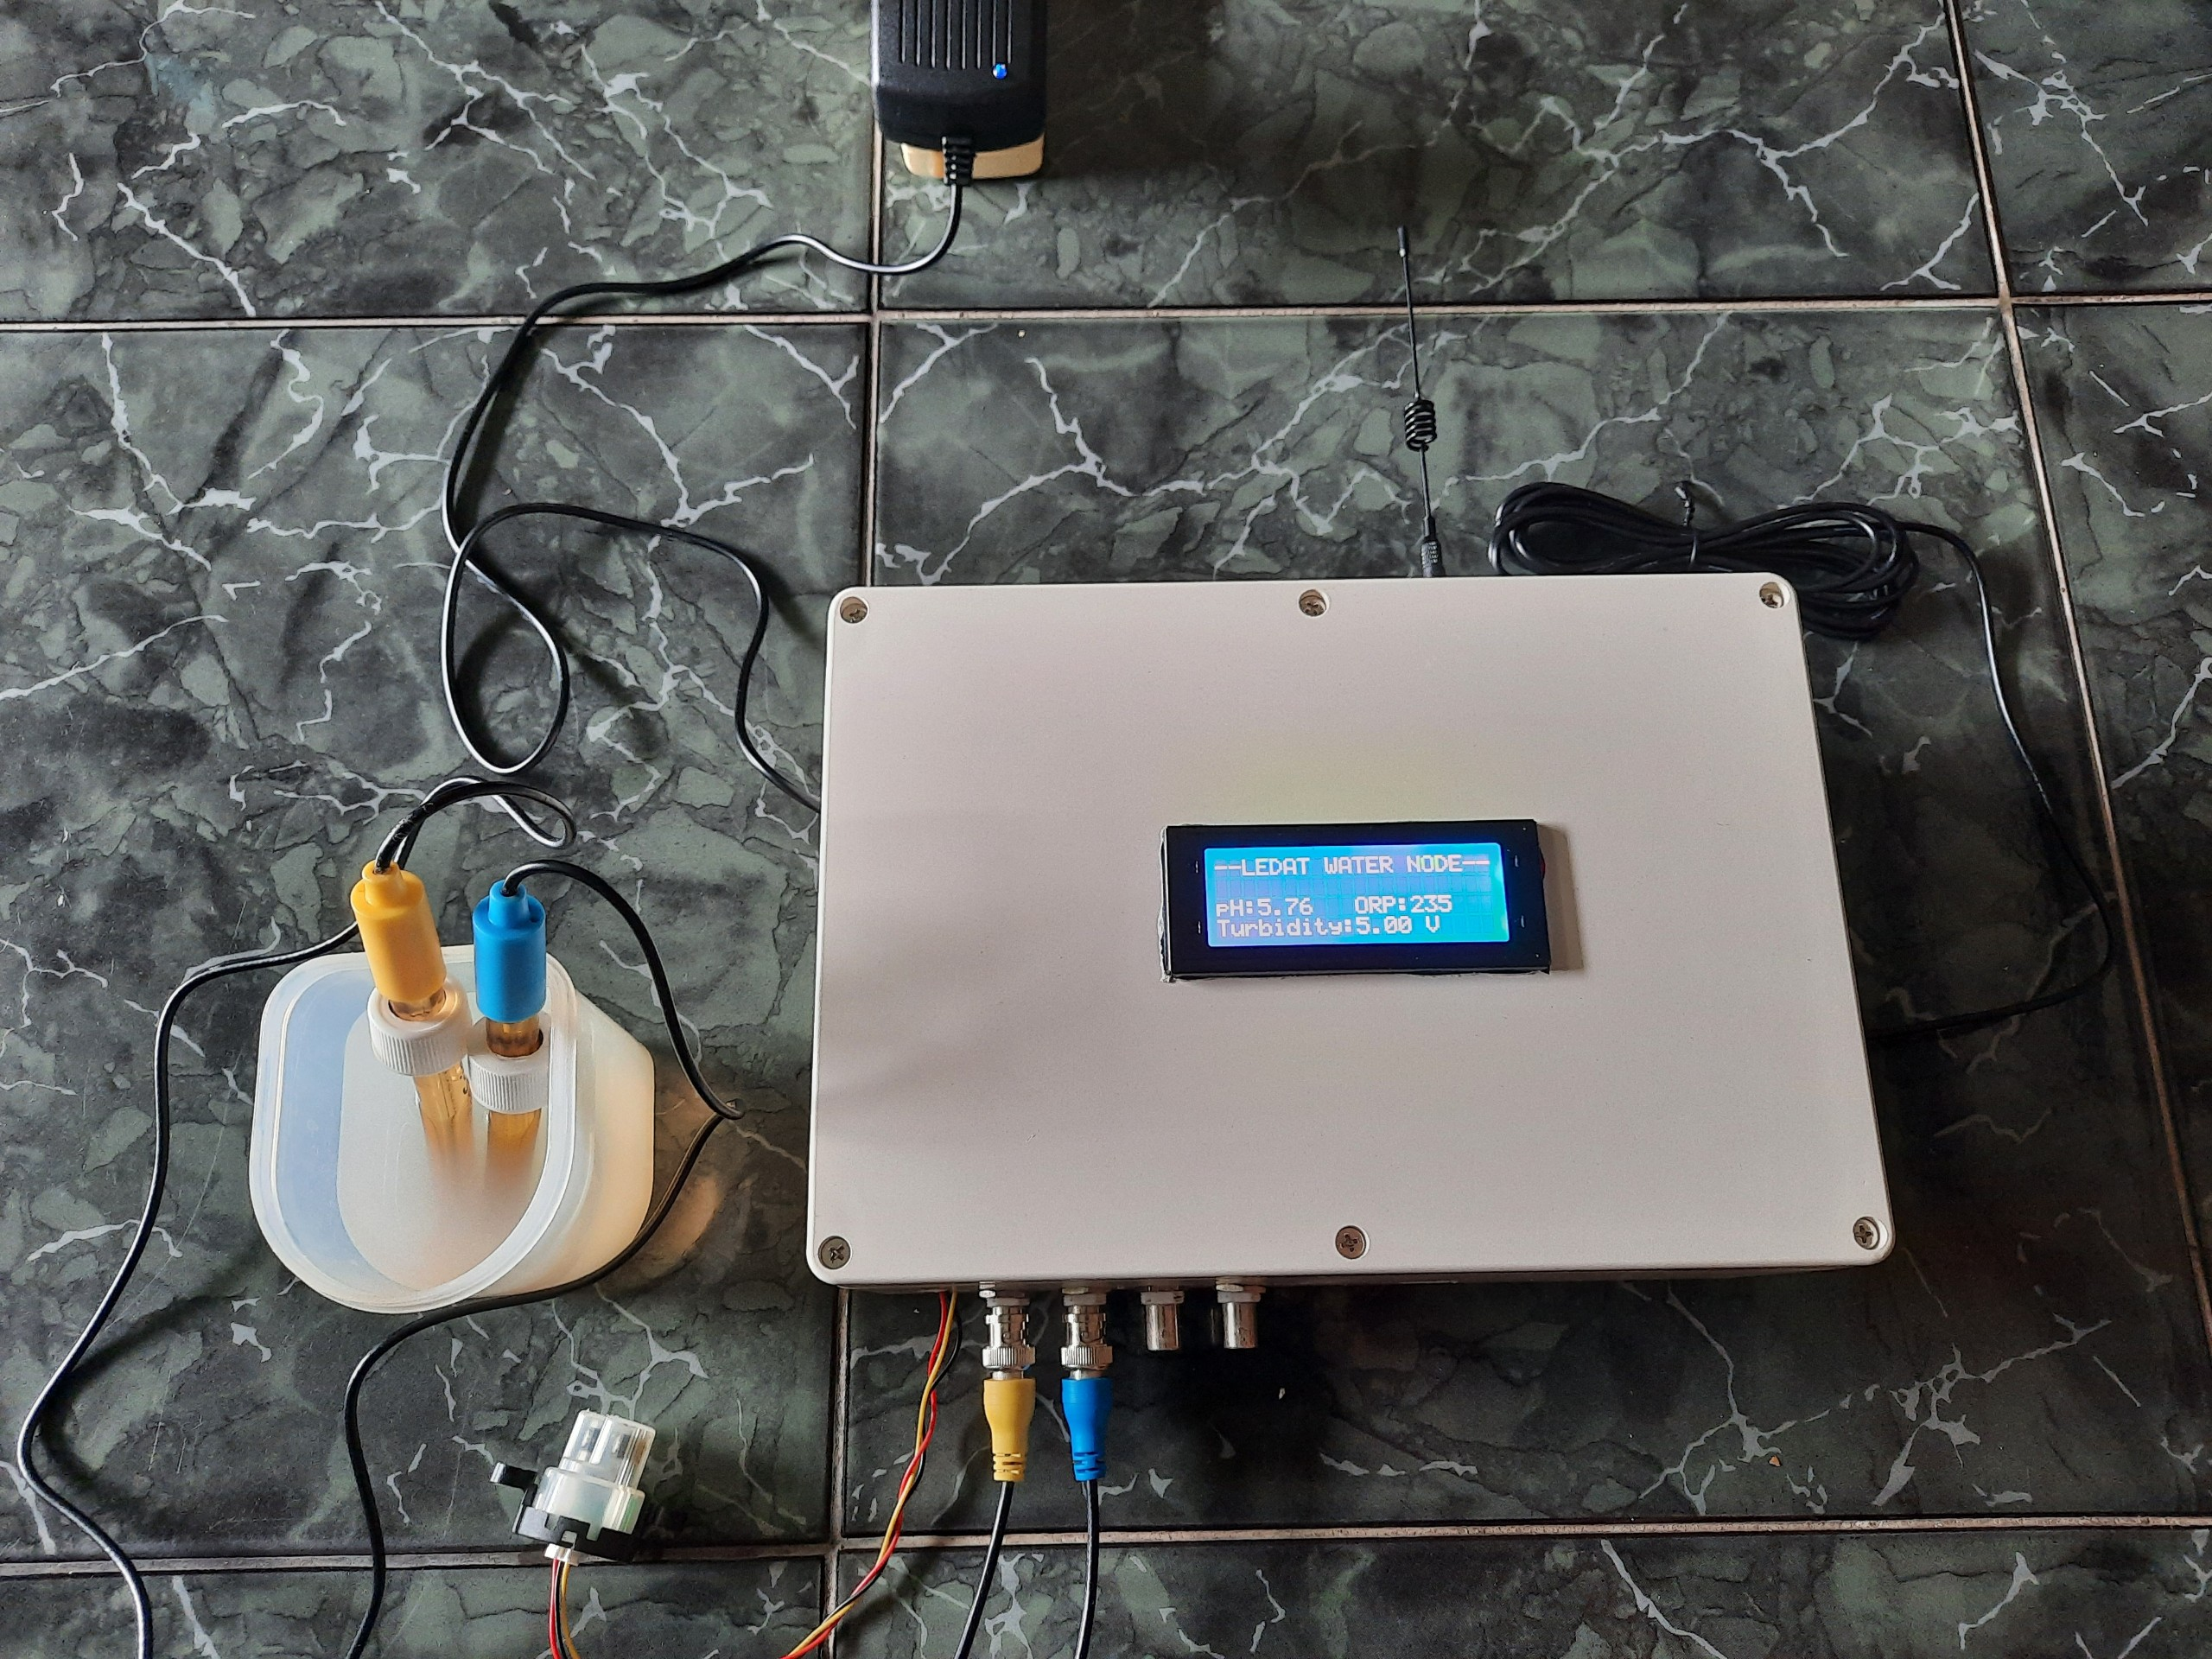
\includegraphics[scale=0.1]{Chapter 4/image chapter 4/aotomNode.jpg}
	\caption[Phần cứng node ao tôm thực tế]{Phần cứng node ao tôm thực tế}
\end{figure}
\indent Anten được bố trí phía trên hộp để đảm bảo node có thể truyền nhận dữ liệu 1 cách tốt nhất, Anten đã được nâng cấp lên Anten GSM 9dbi SMA Đực để tăng khả năng giao tiếp. Trong tương lai, em cũng sẽ nâng cấp anten của node vườn thanh long tương tự như vậy.
\begin{figure}[H]
	\centering
	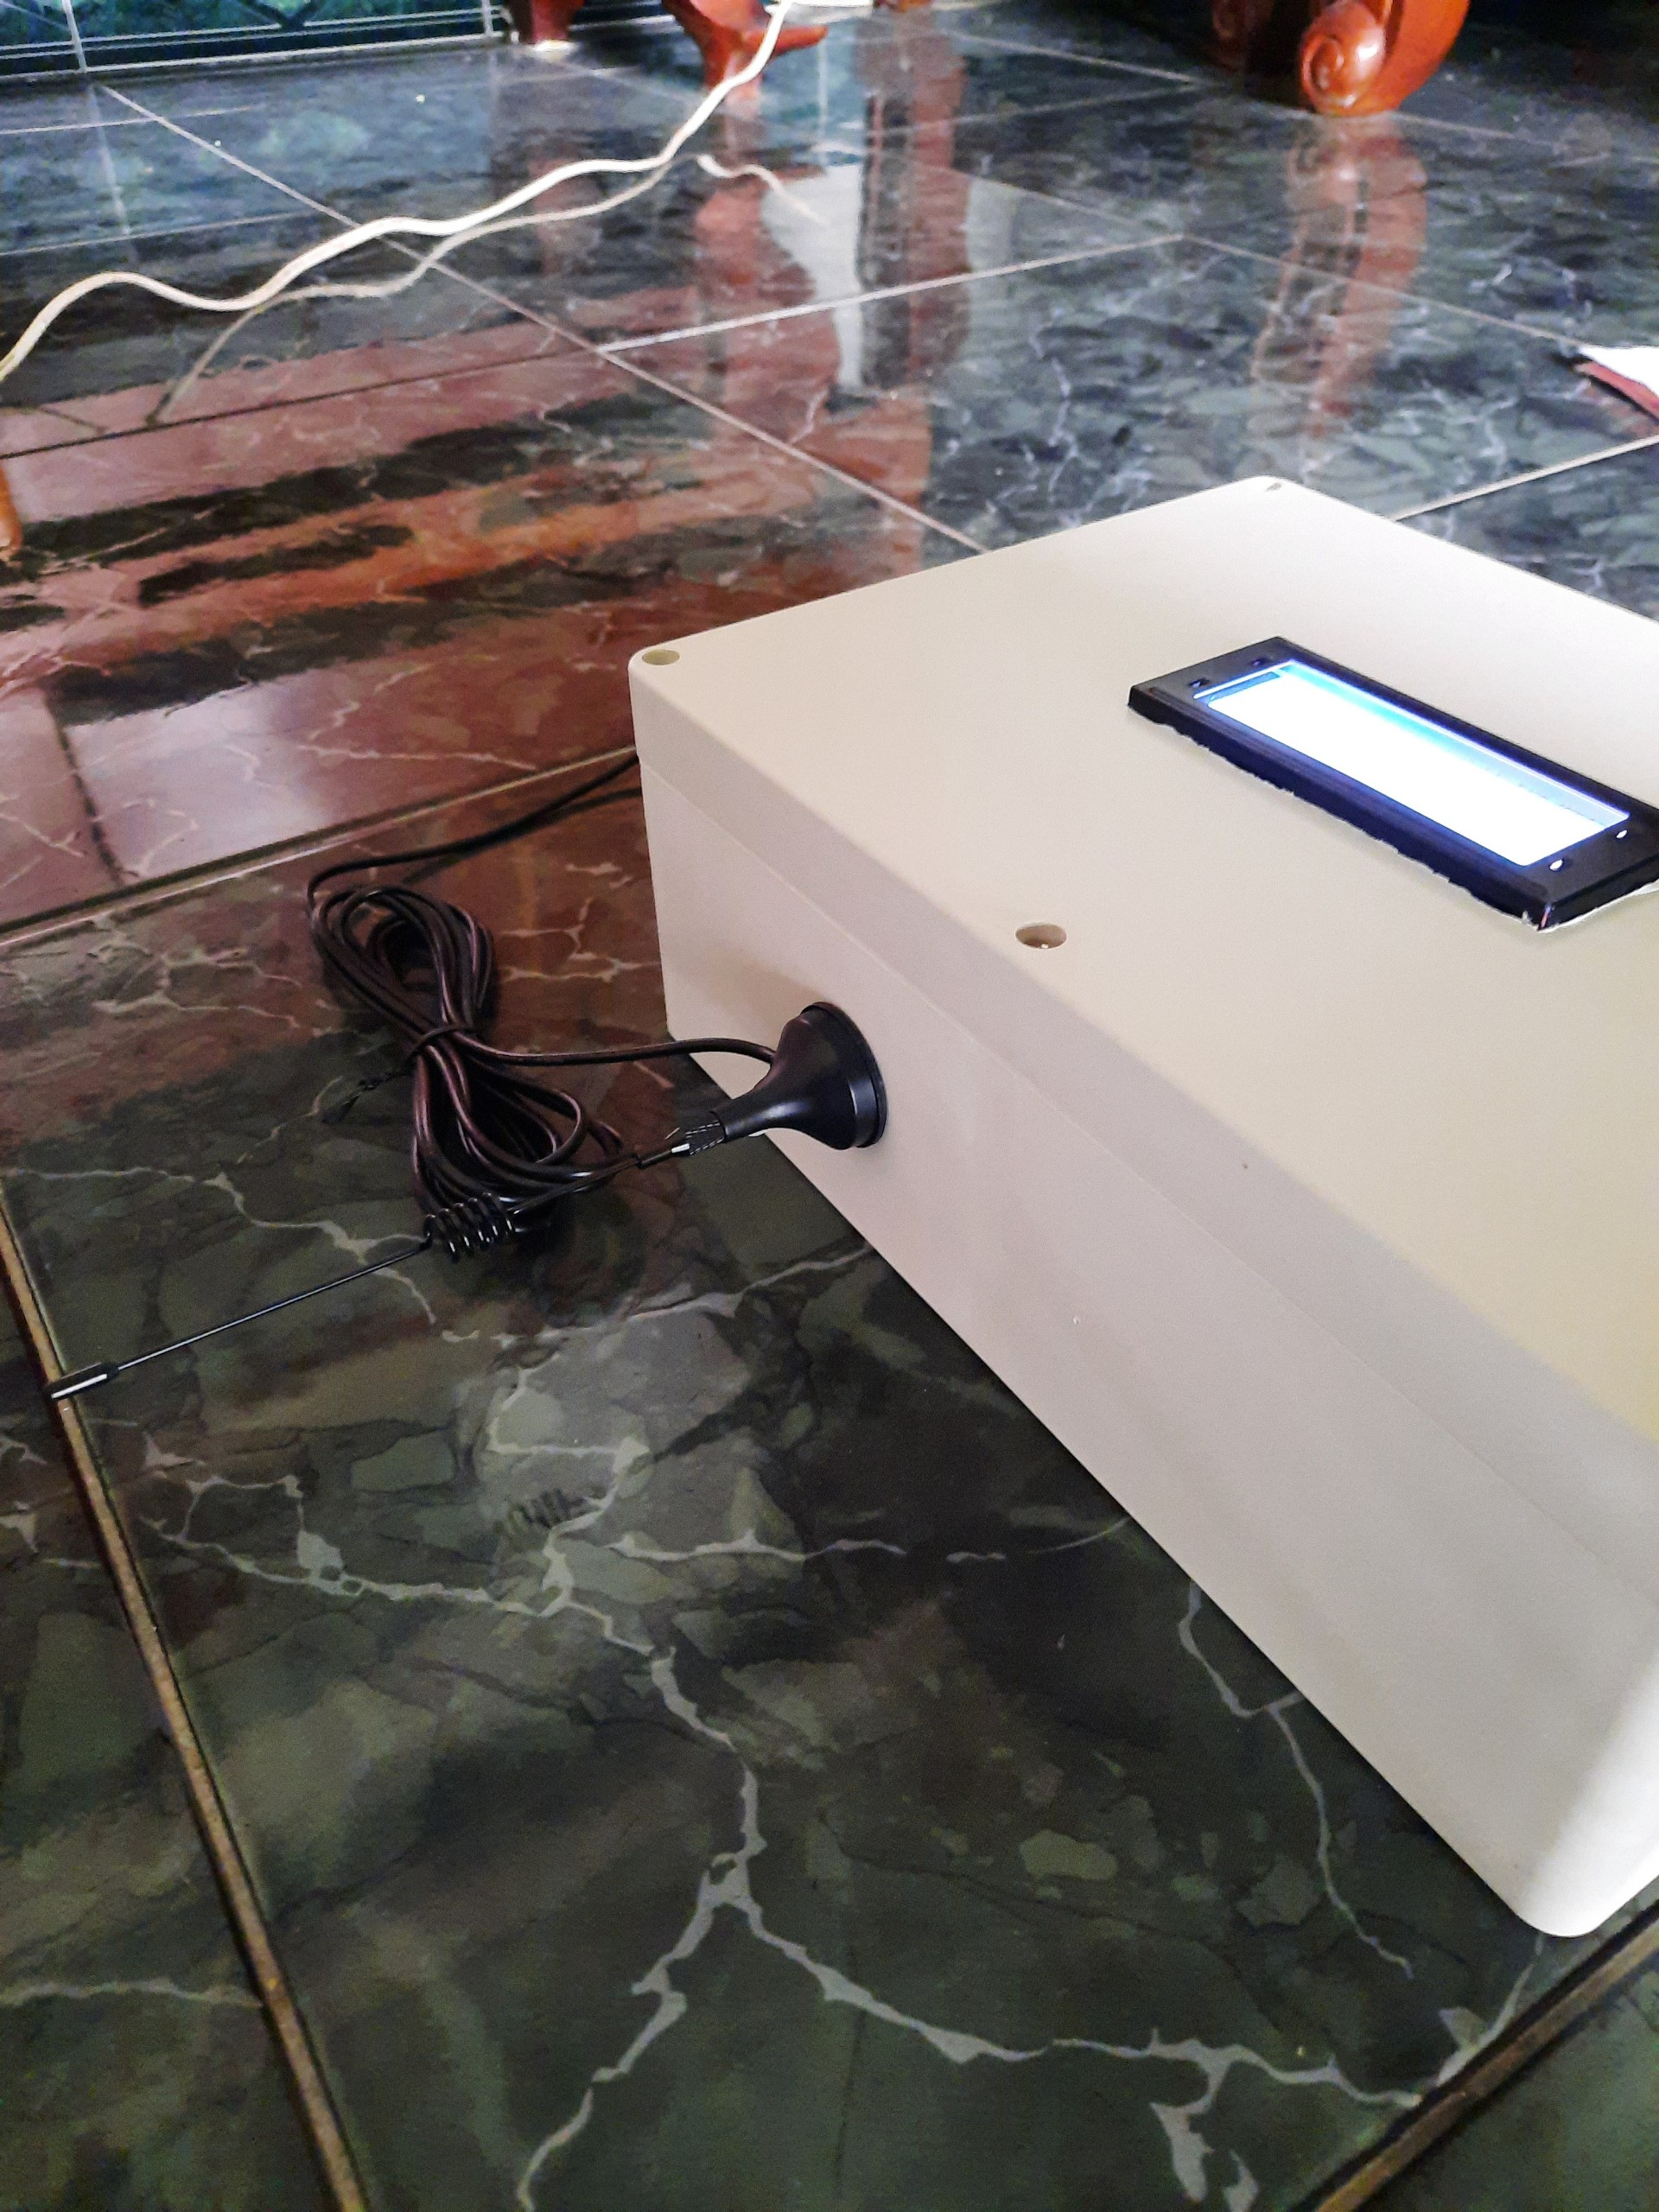
\includegraphics[scale=0.1]{Chapter 4/image chapter 4/antenAotom.jpg}
	\caption[Phần cứng node ao tôm thực tế]{Phần cứng node ao tôm thực tế}
\end{figure}
\subsection{KIỂM TRA CÁC THÔNG SỐ MÔI TRƯỜNG THU ĐƯỢC TỪ 2 NODE}
Dưới đây là hình ảnh được hiển thị trên App và Gateway cho ta biết các giá trị được 2 node Arduino thu về từ cảm biến và truyền lại cho gateway thông qua sóng LoRa.\\
\indent Với các thông số của môi trường thu về được từ 2 node như sau:
\begin{itemize}
	\item \textbf{\textit{Nhiệt độ: }} 33*C
	\item \textbf{\textit{Độ ẩm không khí: }} 61\%
	\item \textbf{\textit{Độ ẩm đất: }} 0\% (do cảm biến độ ẩm đất chưa được cắm vào đất)
	\item \textbf{\textit{Độ pH của nước: }} 4.59 (môi trường thử nghiệm là môi trường xà phòng)
	\item \textbf{\textit{Chỉ số oxi hoá khử: }} 279
	\item \textbf{\textit{Độ đục của nước: }} -4352.9 NTU (do cảm biến đang được đặt trên môi trường không khí chưa được cho vào môi trường nước đục)
\end{itemize}

\begin{figure}[H]
	\centering
	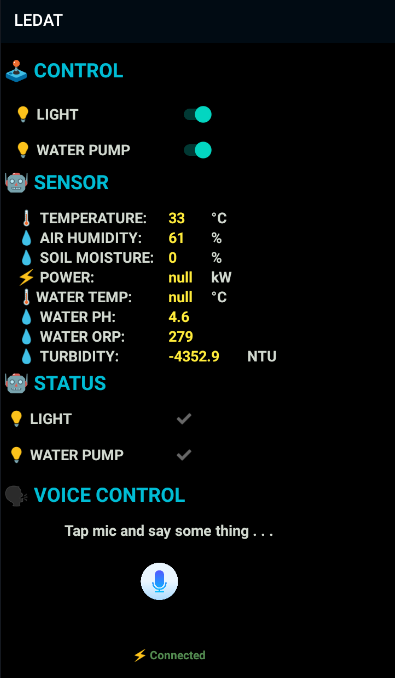
\includegraphics[scale=0.4]{Chapter 4/image chapter 4/appMT.png}
	\caption[Các thông số của môi trường được hiển thị trên app]{Các thông số của môi trường được hiển thị trên app}
	\label{hinh43}
\end{figure}
\begin{figure}[H]
	\centering
	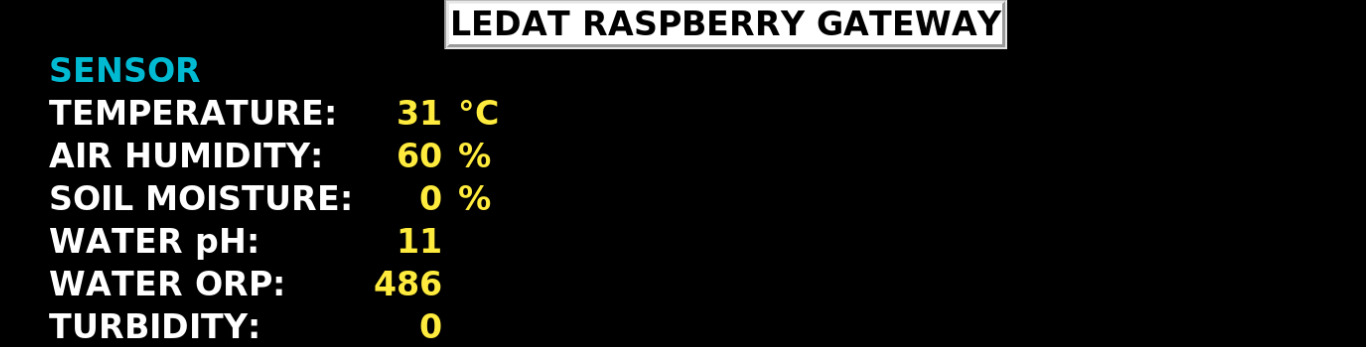
\includegraphics[scale=0.4]{Chapter 4/image chapter 4/gwMT.png}
	\caption[Các thông số của môi trường được hiển thị trên Gateway]{Các thông số của môi trường được hiển thị trên Gateway}
	\label{hinh44}
\end{figure}
\subsection{KIỂM TRA HOẠT ĐỘNG CỦA NODE AO TÔM}
\indent Các thông số từ cảm biến được hiển thiện trên màn hình LCD 20x4 tiện lợi cho việc theo dõi trực tiếp các thông số mà không cần thông qua quan sát trên Gateway.
\begin{figure}[H]
	\centering
	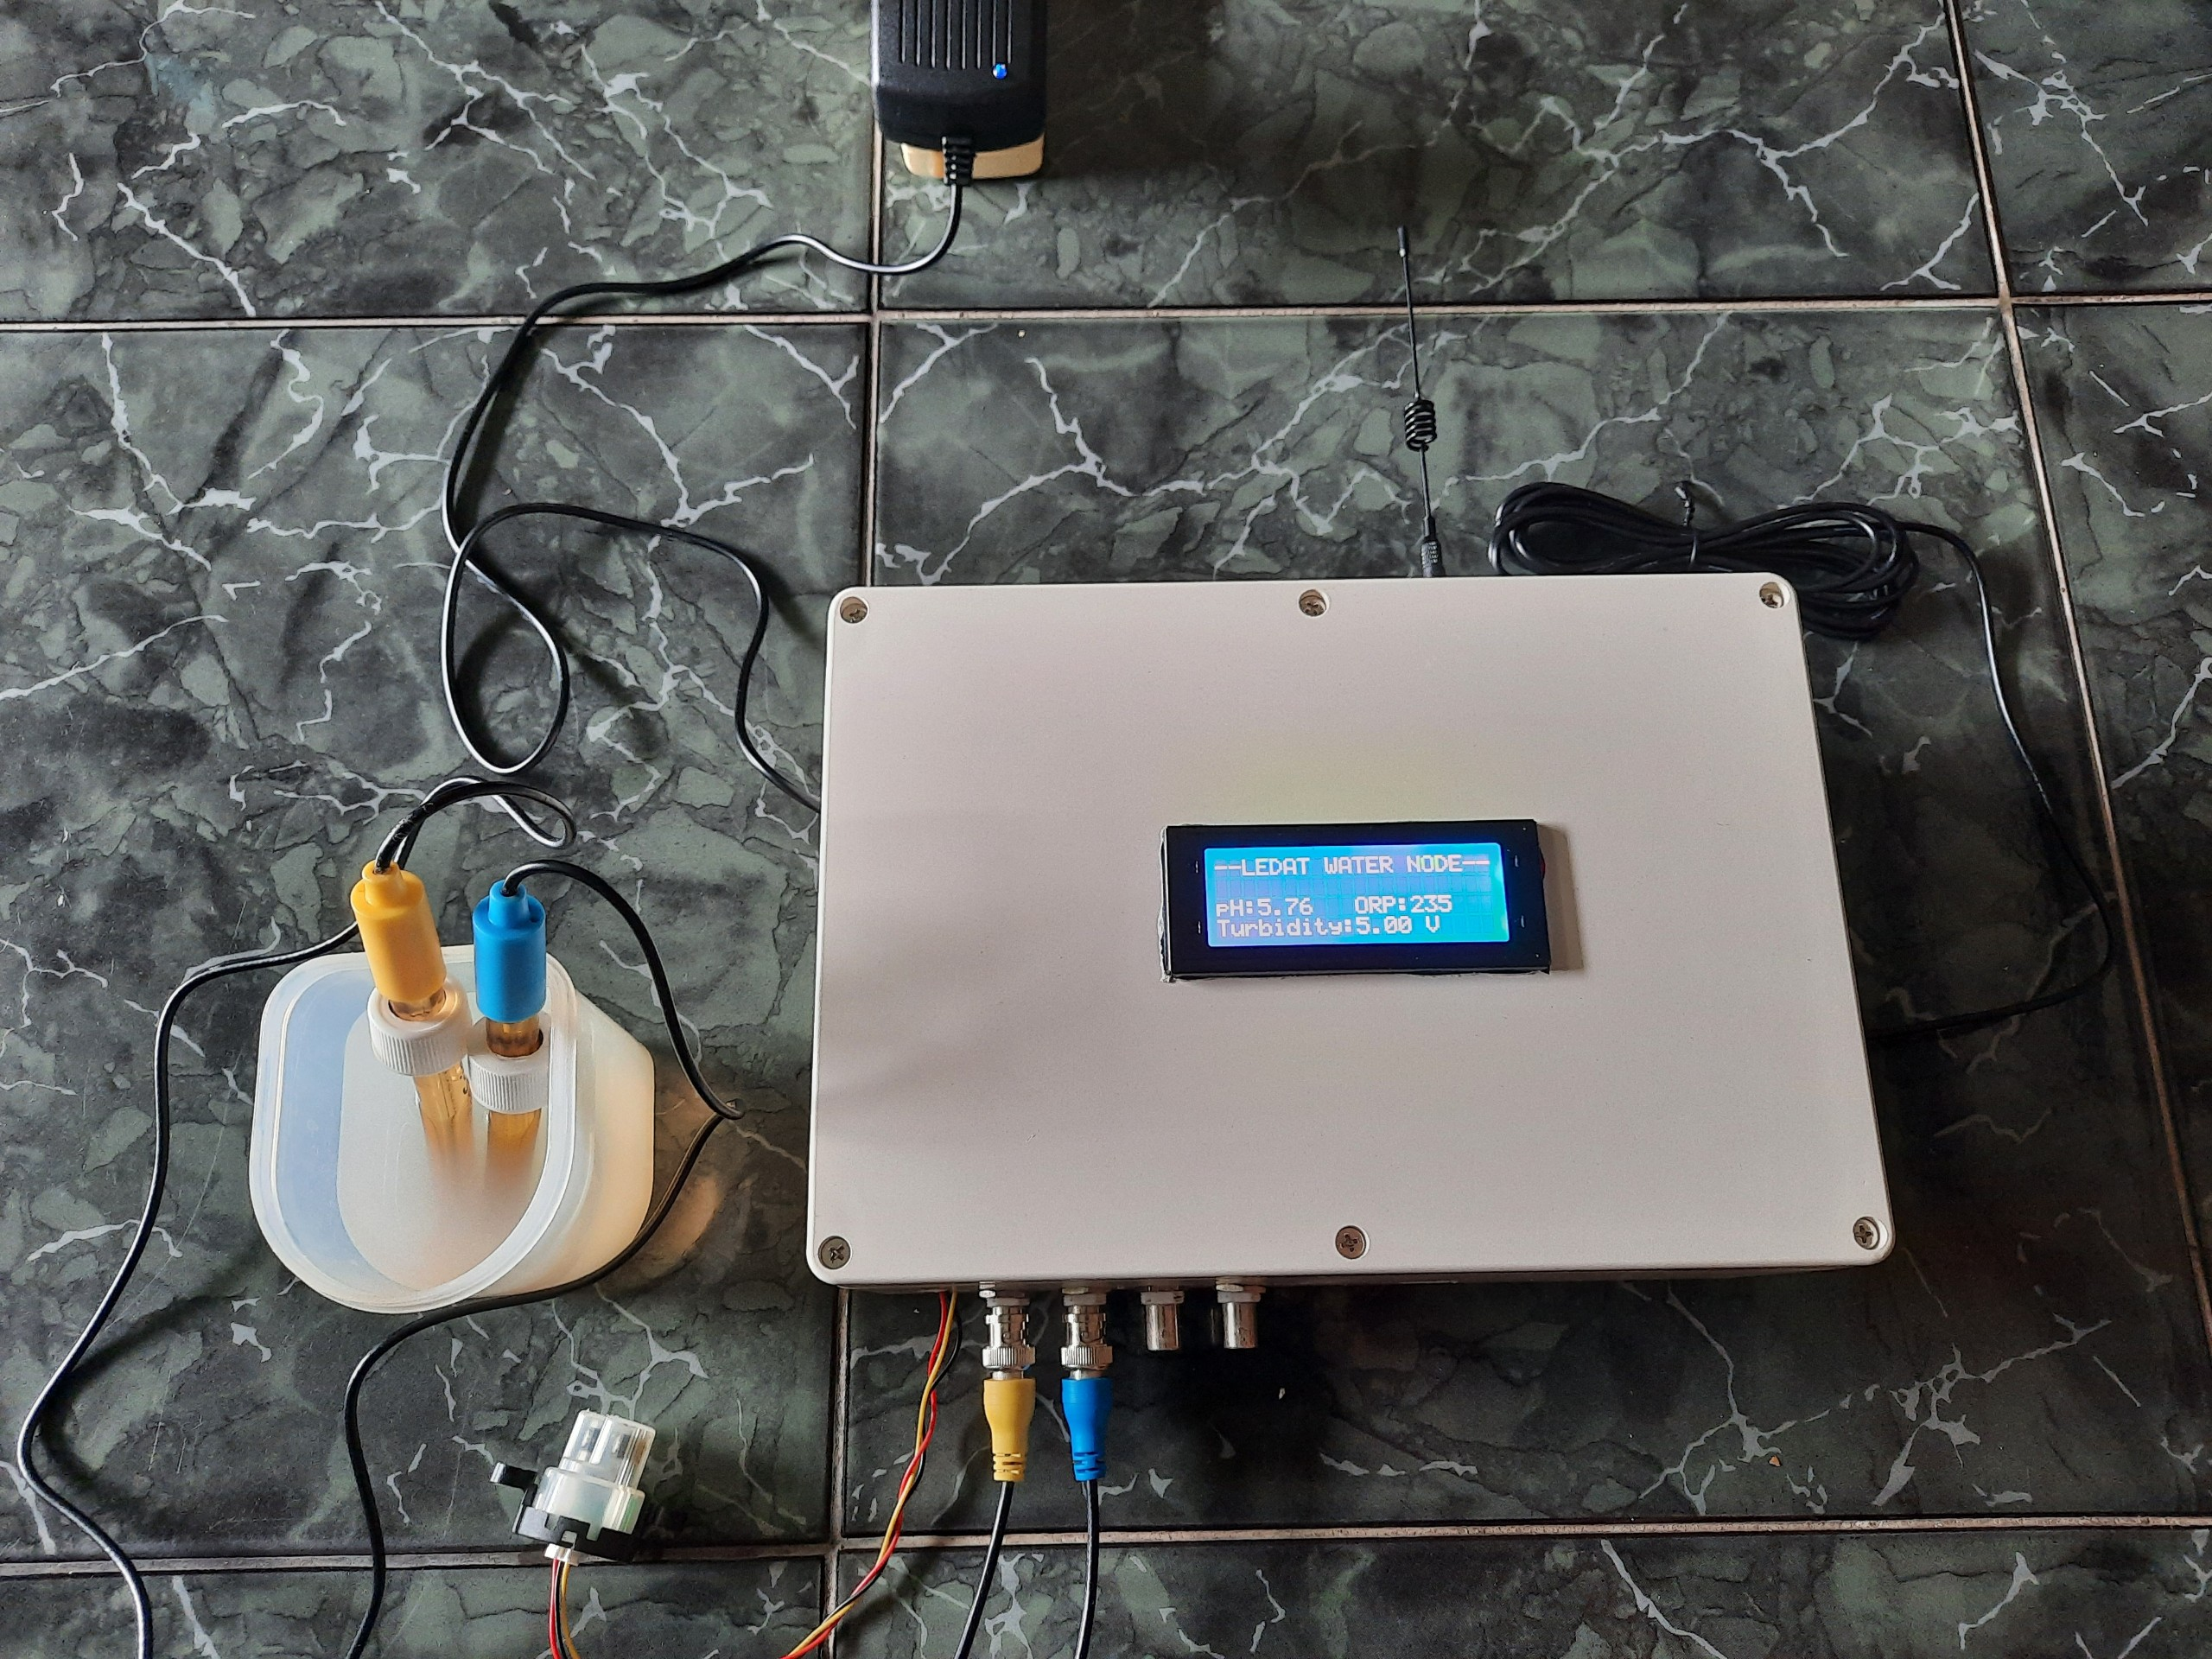
\includegraphics[scale=0.1]{Chapter 4/image chapter 4/aotomNode.jpg}
	\caption[Các thông số của môi trường nước được cảm biến thu về và hiển thị trên màn hình LCD]{Các thông số của môi trường nước được cảm biến thu về và hiển thị trên màn hình LCD}
\end{figure}
\subsection{KIỂM TRA HOẠT ĐỘNG CỦA MODULE 2 RELAY}
Ta tiến hành thử nghiệm bằng cách bật relay 1. Dưới đây là hình ảnh phần cứng phản hồi lại lệnh điều khiển bật relay 1 nhận từ Gateway truyền về thông qua LoRa.
\begin{figure}[H]
	\centering
	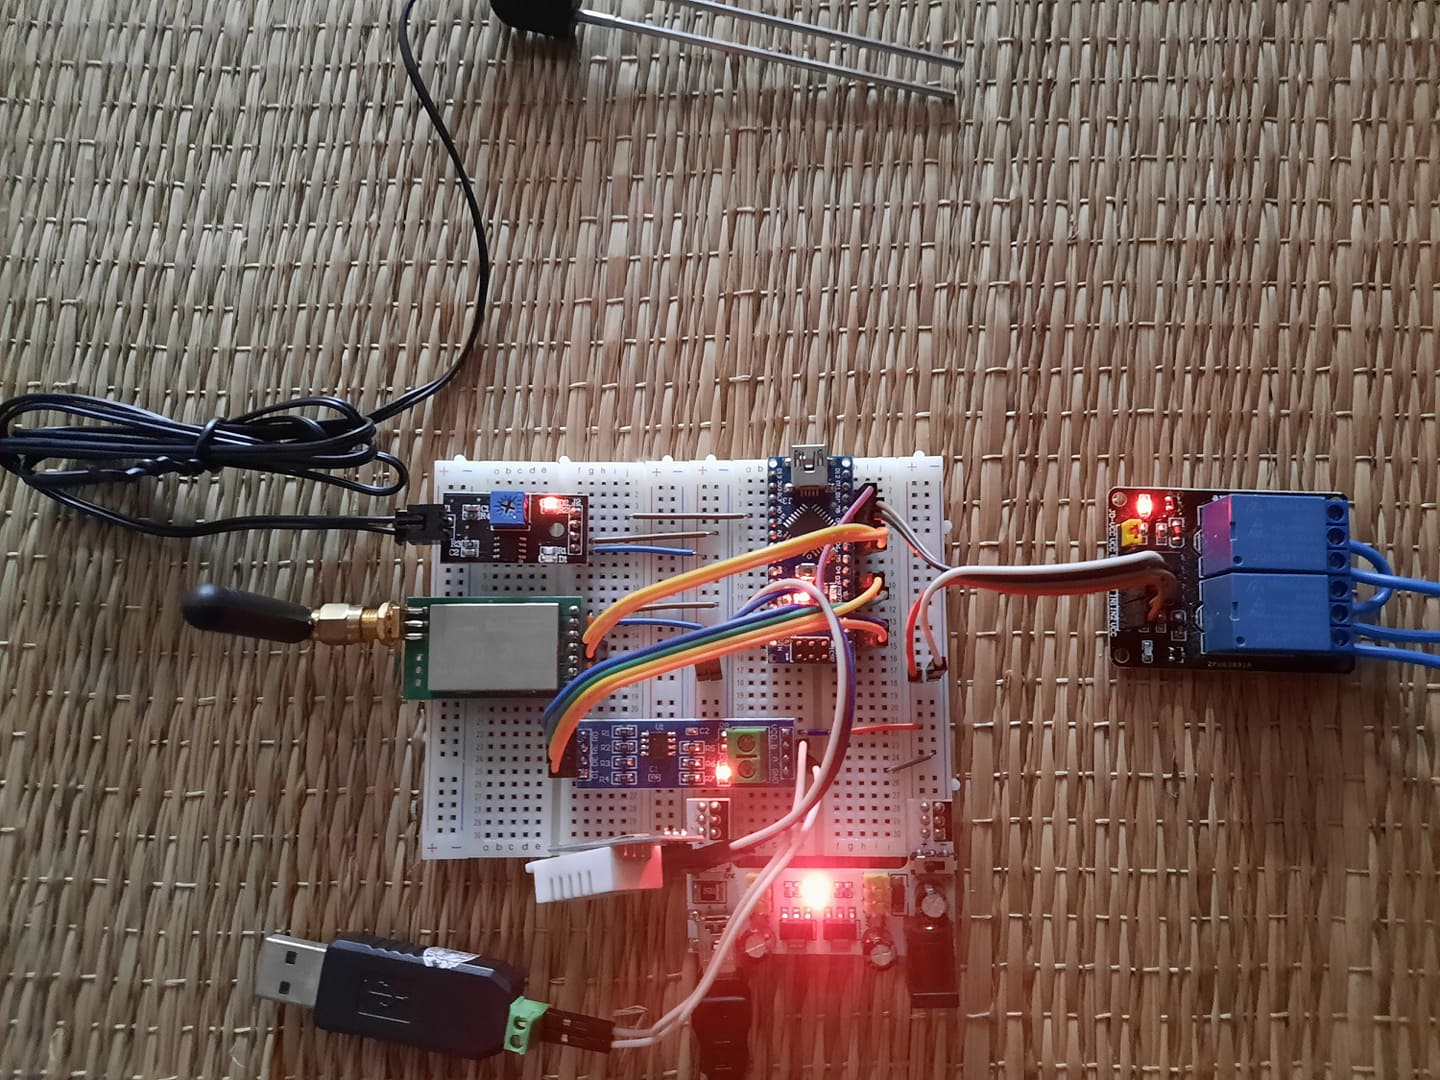
\includegraphics[scale=0.2]{Chapter 4/image chapter 4/R1ONR2OFF.jpg}
	\caption[Phần cứng trong trạng thái bật relay 1 tắt relay 2]{Phần cứng trong trạng thái bật relay 1 tắt relay 2}
	\label{hinh45}
\end{figure}
\indent Giao diện trên app đã hiển thị được các thông số của môi trường cũng như trạng thái bật/tắt của 2 thiết bị tại relay 1 và relay 2
\begin{figure}[H]
	\centering
	
\includegraphics[scale=0.2]{Chapter 4/image chapter 4/appR1ONR2OFF.png}
	\caption[Trang thái của end-Node được hiển thị trên app]{Trang thái của end-Node được hiển thị trên app}
	\label{hinh46}
\end{figure}
\indent Giao diện trên Gateway cũng đã hiển thị được các thông số của môi trường và trạng thái của 2 relay.
\begin{figure}[H]
	\centering
	
\includegraphics[scale=0.3]{Chapter 4/image chapter 4/Relay1ON-Relay2OFF.png}
	\caption[Trang thái của end-Node được hiển thị trên Gateway]{Trang thái của end-Node được hiển thị trên Gateway}
	\label{hinh47}
\end{figure}
\indent Tương tự, ta tiến hành thử nghiệm bật relay 2 và tắt relay 1.
\begin{figure}[H]
	\centering
	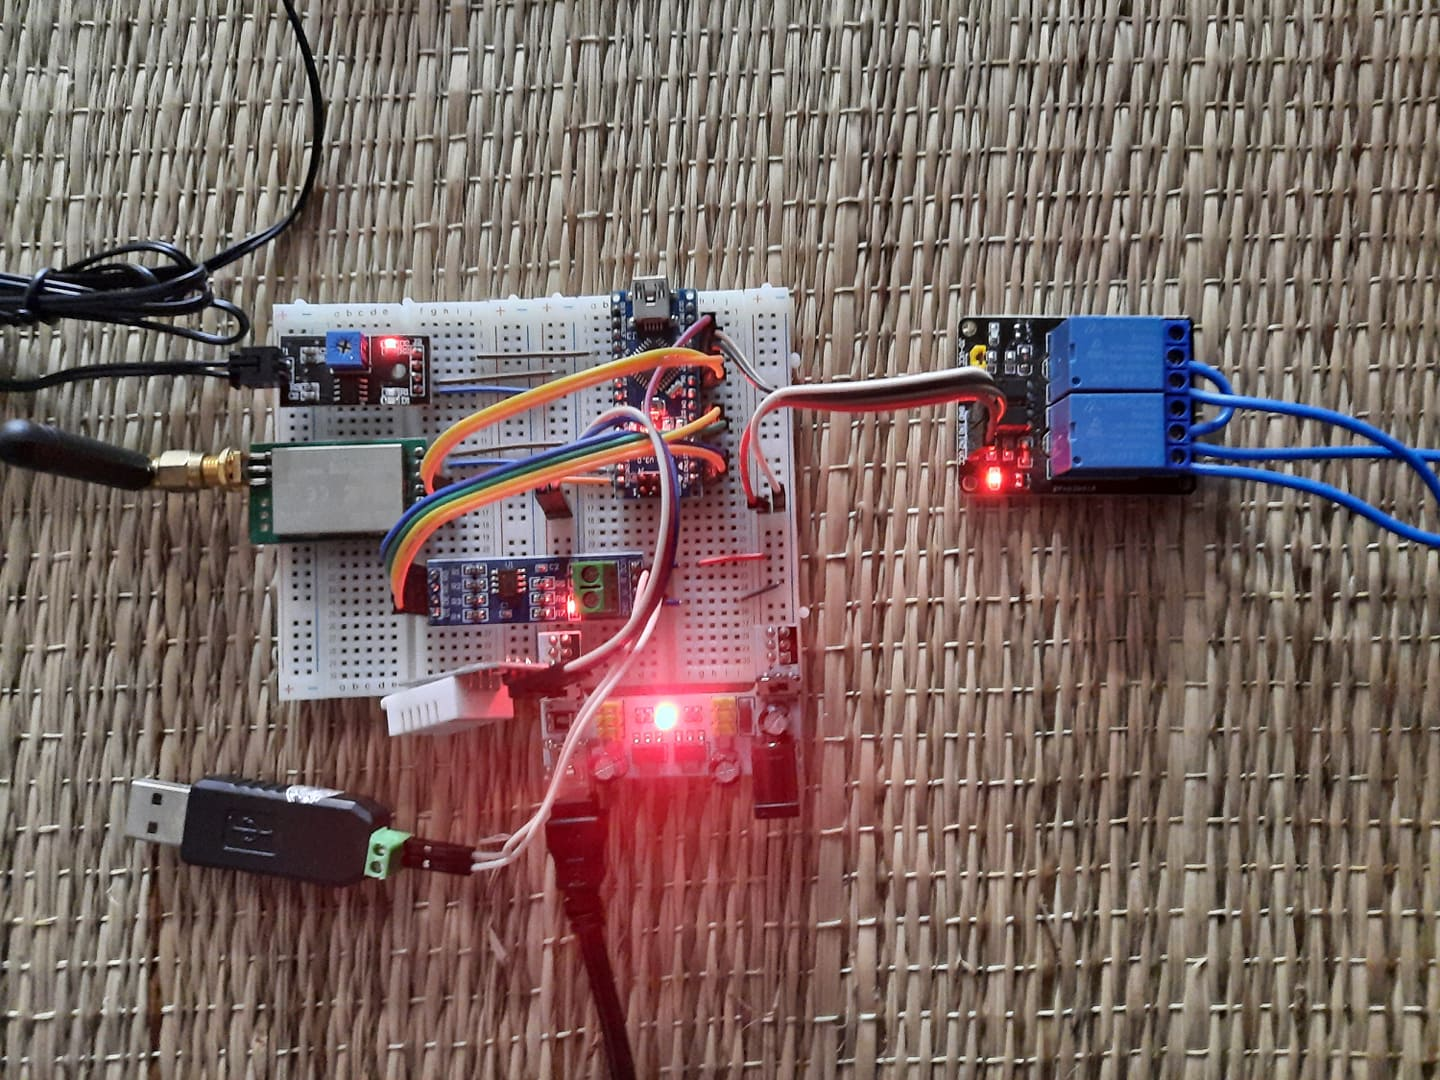
\includegraphics[scale=0.2]{Chapter 4/image chapter 4/R2ONR1OFF.jpg}
	\caption[Phần cứng trong trạng thái bật relay 2 tắt relay 1]{Phần cứng trong trạng thái bật relay 2 tắt relay 1}
	\label{hinh48}
\end{figure}
\begin{figure}[H]
	\centering
	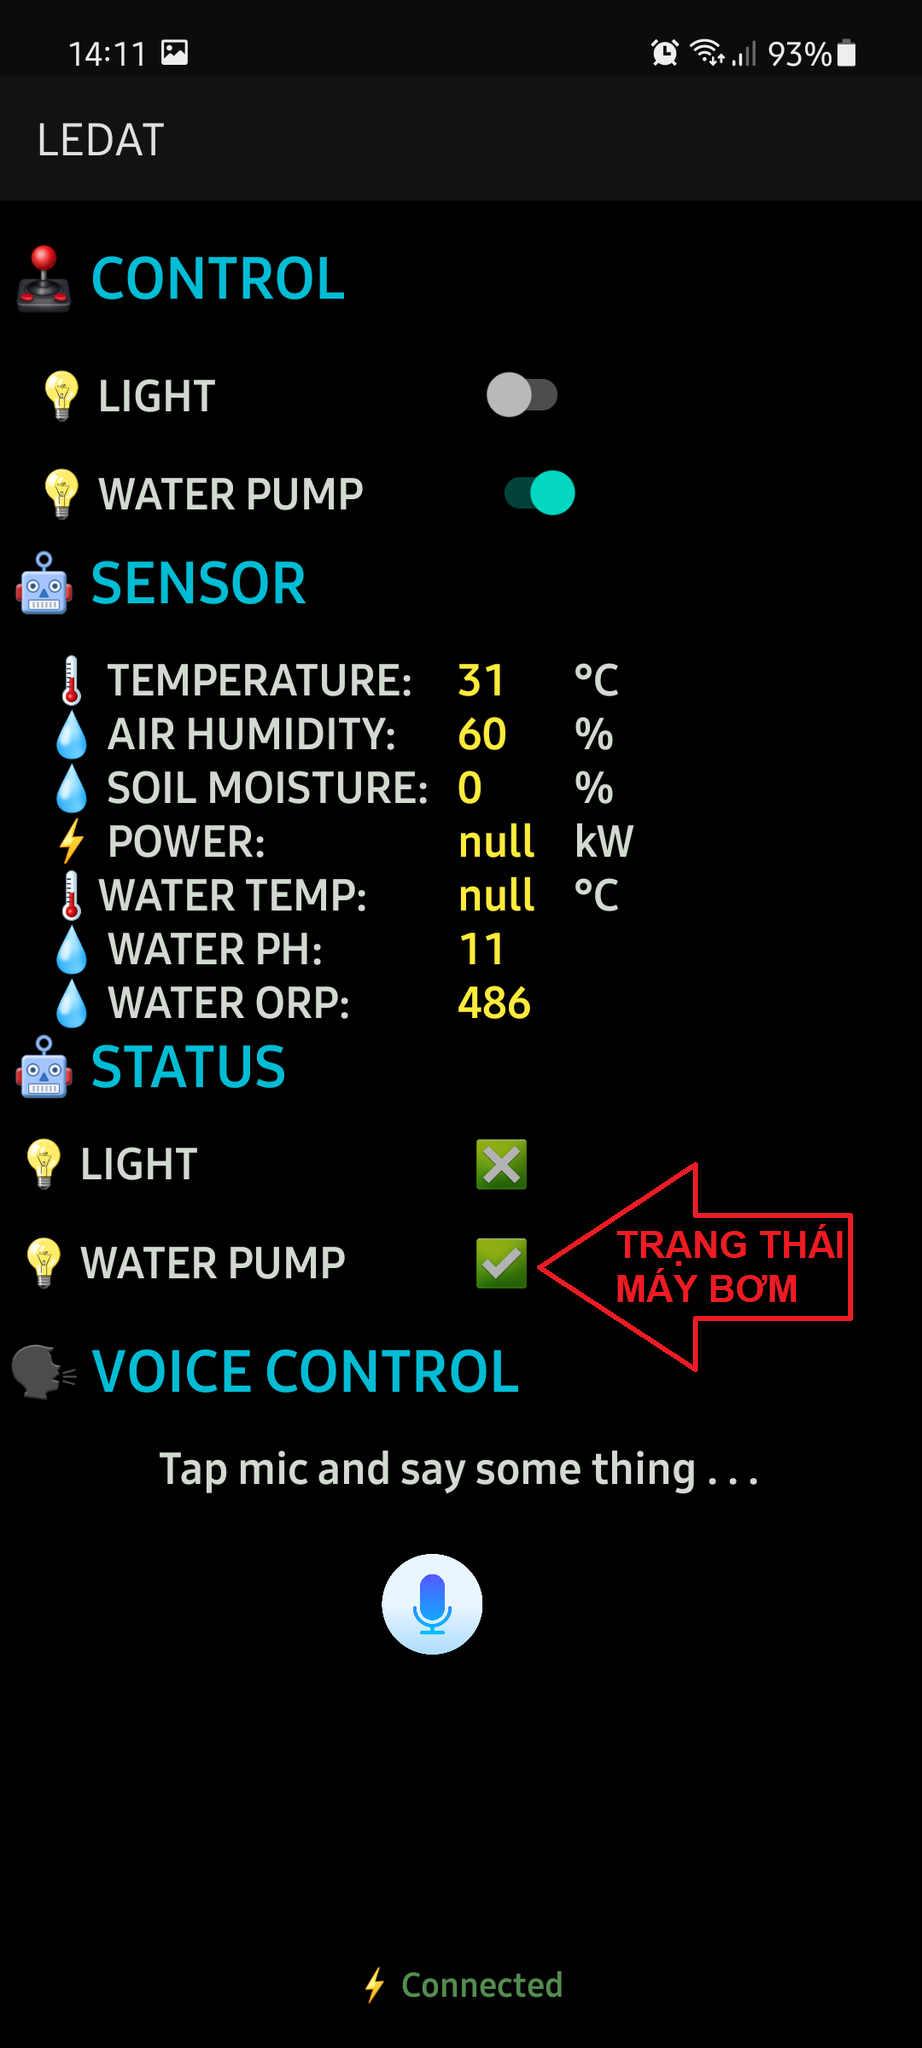
\includegraphics[scale=0.2]{Chapter 4/image chapter 4/appR1OFFR2ON.png}
	\caption[Trang thái của end-Node được hiển thị trên app]{Trang thái của end-Node được hiển thị trên app}
	\label{hinh49}
\end{figure}
\begin{figure}[H]
	\centering
	
\includegraphics[scale=0.3]{Chapter 4/image chapter 4/Relay1OFF-Relay2ON.png}
	\caption[Trang thái của end-Node được hiển thị trên Gateway]{Trang thái của end-Node được hiển thị trên Gateway}
	\label{hinh410}
\end{figure}

\section*{CHƯƠNG 5: KẾT LUẬN VÀ HƯỚNG PHÁT TRIỂN}
\addcontentsline{toc}{section}{\numberline {} CHƯƠNG 5: KẾT LUẬN VÀ HƯỚNG PHÁT TRIỂN}
\setcounter{section}{5}
\setcounter{subsection}{0}
\subsection{KẾT LUẬN}
Sản phẩm gửi dữ liệu và phản hồi lệnh điều khiển từ Gateway rất tốt, không xảy ra hiện tượng mất dữ liệu, các thông số nhiệt độ và độ ẩm cũng rất sát với thực tế, tuy nhiên hệ thống vẫn hoạt động thời gian dài vẫn chưa ổn định do xảy ra hiên tượng crash trên Gataway, cụ thể là lỗi ép kiểu dữ liệu.
\subsection{HƯỚNG PHÁT TRIỂN}
Nâng cao tính ổn định cho hệ thống, thêm các cảm biến nếu cần thiết.

\section*{TÀI LIỆU THAM KHẢO}
\addcontentsline{toc}{section}{\numberline {} TÀI LIỆU THAM KHẢO}
[1]. Nguyễn Văn Quảng - Nguyễn Tài. (2018). TÌM HIỂU NGUYÊN LÝ HOẠT ĐỘNG CỦA CÁC MODULE DÙNG CÔNG NGHỆ LORA\\
\indent [2]. \textit{Khái niệm cơ bản về LoRa}. Truy cập từ:\\
\indent \url{https://bkaii.com.vn/tin-tuc/135-khai-niem-co-ban-ve-lora}\\
\indent [3]. \textit{MQTT là gì? Vai trò của MQTT trong IoT}. Truy cập từ:\\
\indent \url{https://viblo.asia/p/mqtt-la-gi-vai-tro-cua-mqtt-trong-iot-V3m5WL3bKO7}\\
\indent [4]. Hshop. Truy cập từ: \url{https://hshop.vn/}


\end{document}
